\documentclass{article}
\usepackage{graphicx} % Required for inserting images
\usepackage[nonumberlist]{glossaries}
\usepackage[italian]{babel}
\usepackage{hyperref}
\usepackage[noabbrev]{cleveref}
\usepackage{biblatex}
\usepackage{comment}

\usepackage{bera}% optional: just to have a nice mono-spaced font
\usepackage{listings}
\usepackage{xcolor}
\usepackage{float}

\usepackage{geometry}
 \geometry{
     margin=1in,
     a4paper,
     total={170mm,240mm},
     left=25mm,
     top=20mm,
 }

\colorlet{punct}{red!60!black}
\definecolor{background}{HTML}{EEEEEE}
\definecolor{delim}{RGB}{20,105,176}
\colorlet{numb}{magenta!60!black}

\lstdefinelanguage{json}{
    basicstyle=\normalfont\ttfamily,
    numbers=left,
    numberstyle=\scriptsize,
    stepnumber=1,
    numbersep=8pt,
    showstringspaces=false,
    breaklines=true,
    frame=lines,
    backgroundcolor=\color{background},
    literate=
     *{0}{{{\color{numb}0}}}{1}
      {1}{{{\color{numb}1}}}{1}
      {2}{{{\color{numb}2}}}{1}
      {3}{{{\color{numb}3}}}{1}
      {4}{{{\color{numb}4}}}{1}
      {5}{{{\color{numb}5}}}{1}
      {6}{{{\color{numb}6}}}{1}
      {7}{{{\color{numb}7}}}{1}
      {8}{{{\color{numb}8}}}{1}
      {9}{{{\color{numb}9}}}{1}
      {:}{{{\color{punct}{:}}}}{1}
      {,}{{{\color{punct}{,}}}}{1}
      {\{}{{{\color{delim}{\{}}}}{1}
      {\}}{{{\color{delim}{\}}}}}{1}
      {[}{{{\color{delim}{[}}}}{1}
      {]}{{{\color{delim}{]}}}}{1},
}

\lstdefinestyle{yaml}{
     basicstyle=\color{blue}\footnotesize,
     rulecolor=\color{black},
     string=[s]{'}{'},
     stringstyle=\color{blue},
     comment=[l]{\#},
     commentstyle=\color{black},
     morecomment=[l]{-}
 }

\usepackage{forest}

\definecolor{folderbg}{RGB}{124,166,198}
\definecolor{folderborder}{RGB}{110,144,169}

\def\Size{4pt}
\tikzset{
      folder/.pic={
        \filldraw[draw=folderborder,top color=folderbg!50,bottom color=folderbg]
          (-1.05*\Size,0.2\Size+5pt) rectangle ++(.75*\Size,-0.2\Size-5pt);  
        \filldraw[draw=folderborder,top color=folderbg!50,bottom color=folderbg]
          (-1.15*\Size,-\Size) rectangle (1.15*\Size,\Size);
      }
    }

\crefformat{section}{\S#2#1#3}
\crefformat{subsection}{\S#2#1#3}
\crefformat{subsubsection}{\S#2#1#3}
\crefformat{figure}{#2Figura~#1#3}
\crefformat{lstlisting}{#2Listato~#1#3}
\crefformat{footnote}{#2\footnotemark[#1]#3}
\crefformat{table}{#2Tabella~#1#3}
\crefformat{equation}{#2Equazione~#1#3}
\crefformat{chapter}{#2Capitolo~#1#3}

\addbibresource{refs.bib}

\renewcommand{\contentsname}{Indice}

\makeglossaries

\newglossaryentry{player} 
{  
    name={player (\textmd{oppure} giocatore)},
    text=giocatore,
    description=è l'entità che può eseguire un turno nei round di un game. 
}

\newglossaryentry{game}
{
    name={game (\textmd{oppure} gioco, partita)},
    text=partita,
    description={è l'entità principale del sistema. Un game è composto da più round}
}

\newglossaryentry{round}
{
    name=round,
    text=round,
    description={è l'entità che contiene le informazioni di gioco principali. Ogni game è composto da un numero 
    finito di round durante il quale ciascun giocatore effettua la propria giocata}
}

\newglossaryentry{turn}
{
    name={turn (\textmd{oppure} turno)},
    text=turno,
    description={è l'unità indivisibile di un round e rappresenta le azioni di un giocatore durante il round. Quindi contiene informazioni sull'esito dell'esecuzione dei test ed i relativi 
    risultati nonché le classi generate per risolvere il problema}
}

\begin{document}

\begin{titlepage}
    \begin{center}
        \vspace*{1cm}
            
        \Huge
        \textbf{Software Architecture Design}
            
        \vspace{0.5cm}
        \LARGE
        Game Repository - Relazione finale
        
        \vfill
        \vspace{0.8cm}
        
        \Large
        Angelino Pasquale - M63001481 \\
        Capasso Giuseppe -  M63001498 \\
        Dinetti Andrea -  M63001496

    \end{center}
\end{titlepage}

\thispagestyle{empty}

\printglossaries

\newpage
\thispagestyle{empty}
\tableofcontents

\newpage
\thispagestyle{empty}

\begin{comment}
    
DIAGRAMMI DA REALIZZARE:
\begin{itemize}
    \item Use case OK
    \item storie ? .. primo pdf di overleaf TABELLE
    \item architettura generale  context diagram (?)  OK 
    \item class diagram sdm (System domain model) OK
    \item componenti e connettori diagram OK
    \item sequence diagram: (create game, get games , ) : create game OK ,  recupero punteggi dei robot (GET /robot), aggiorna turni con punteggi e vincitore 
    \item activity diagram che spieghi il flusso intero di una partita (games, rounds, turns ...) OK
    \item deployment diagram OK
    \item interface diagram  SWAGGER ?
    \item  ER OK
    \item combinare activity  e sequence in vista  OK
    \item pattern: Facade , singleton, factory, dependency injection , 
    
\end{itemize}



CAPITOLI: 
-Introduzione 
    - Contesto
    - Processi adottati
    - Obiettivo -> Task assegnato 
    
-Analisi Requisiti
    -Tabelle che stavano nel primo doc STORIE
    -USE CASE
    
-Progettazione
    -modellazione
    -Pattern utilizzati
    -tecnologie
    -Documentazione API
    
-Implementazione
    -Flusso partita
    -Sequence diagrams
    -Swagger
https://www.overleaf.com/project/648b01ef29bdb558e1e0f1e9
-Deployment 
    -Docker
    -CD
-Test Collaudo
    -Testing codice
    -CI
\end{comment}

\section{Introduzione}
Questo elaborato descrive le metodologie, le fasi di sviluppo e gli artefatti prodotti nel corso Software Architecture Design dell'anno 2022/23 per la realizzazione di un task specifico all'interno del progetto ENACTEST. In particolare, il progetto ha l'obiettivo principale di creare un gioco con lo scopo di promuovere le attività di \textit{testing} e che permetta ai partecipanti di cimentarsi in sfide contro sistemi automatizzati ed, eventualmente, altri giocatori.

\subsection{Caso di studio}
Il caso oggetto di studio durante il corso prevede l'implementazione di un primo scenario di gioco: un giocatore può effettuare una partita contro un singolo avversario robotico testando una singola classe. In particolare, all'atto della creazione della partita, il giocatore sceglie quale \textit{tool} sfidare. In fase preliminare, gli strumenti automatici scelti sono \textbf{EvoSuite} e \textbf{Randoop}.
\begin{comment}

(QUI METTEREI LA PRIMA ARCHITETTURA CHE HANNO DATO LORO)
(IL CONTEXT DIAGRAM LO METTIAMO IN FASE DI PROGETTAZIONE CREANDO UNA SEZIONE INIZIALE "INTRODUZIONE" IN CUI DICIAMO DOPO BRAIN STORMING E COSE DEL GENERE SIAMO ARRIVATI A QUESTO)


Ai fini dello svolgimento dell'attività curricolare è stato proposto uno dei diversi scenari possibili, che prevede la partecipazione di un singolo giocatore nella partita contro un singolo avversario, che consiste nell'insieme dei \textit{tool} di \textit{testing} automatici \textbf{Randoop} e \textbf{EVOsuite}. Ciò nonostante, il team si è impegnato affinché il sistema progettato sia adattabile anche a scenari più avanzati, come la partecipazione di più giocatori.
--------------------------------------
METTERE QUI IL DIAGRAMMA DI CONTESTO CON LA PRIMA ASSUNZIONE DELL
ARCHITETTURA ????
--------------------------------------
\end{comment}

\subsubsection{Task assegnato}
Il task assegnato prevede la progettazione e lo sviluppo dei requisiti relativi al mantenimento delle partite giocate. Di seguito è riportata la formulazione del task: 

"Per ogni partita giocata dal giocatore il sistema deve mantenere lo storico di tale partita, memorizzando l’Id del giocatore, il tipo di partita (primo scenario, secondo scenario...) la data e l’ora di inizio e di termine della partita, la classe testata, l’insieme dei casi di test creati e i relativi risultati, nonché il Robot con cui si è giocato ed i casi di test creati dal Robot con i relativi risultati."

\subsection{Metodologie adottate}
In questa sezione, sono brevemente descritti gli approcci utilizzati durante lo svolgimento del task.

Il lavoro dei team è stato suddiviso in 3 iterazioni, della durata di circa due settimane ciascuna, al termine delle quali ogni gruppo ha presentato , in sessione plenaria, le attività svolte ottenendo dei \textit{feedback}.

Per adeguarsi al ritmo iterativo di sviluppo sono state svolte le seguenti attività:
\begin{itemize}
    \item Allineamento all'inizio dell'iterazione, per la definizione degli obiettivi e dei task;
    \item Allineamento alla fine dell'iterazione, per valutare i feedback ricevuti;
    \item Aggiornamento dei task e della loro assegnazione sul progetto Github (\cref{fig:task});
    \item Collaborazione durante lo sviluppo con strumenti come Visual Studio Code Share (Pair Programming), e lavagne virtuali condivise;    
\end{itemize}

\begin{figure}[H]
    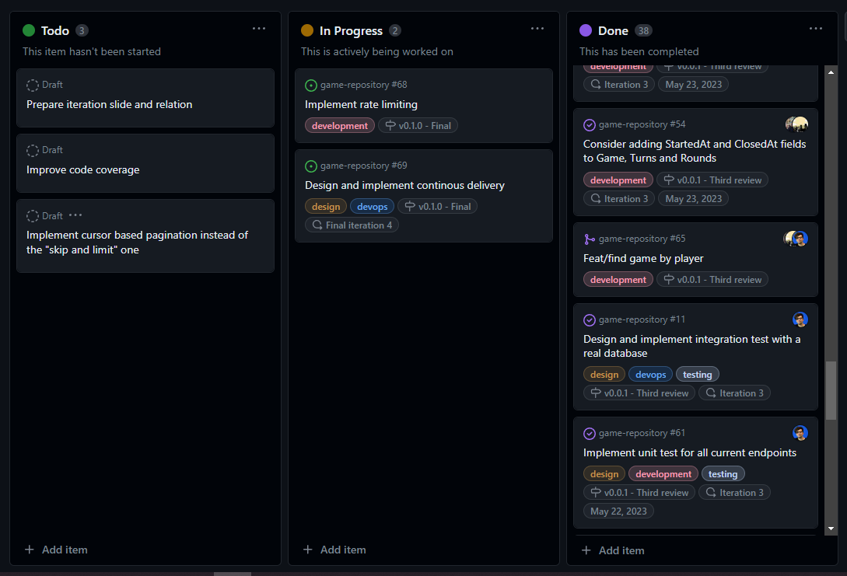
\includegraphics[width=\textwidth]{images/1Introduzione/task.png}
    \caption{Task del progetto}
    \label{fig:task}
\end{figure}

\subsubsection{Link Utili}\label{s:links}
L'applicazione è disponibile in versione demo su questo \href{https://sad.capass.org/docs}{\textbf{link}}.\\

Una guida dettagliata per l'installazione è presente su questo \href{https://testing-game-sad-2023.github.io/T4-G18/}{\textbf{link}}.\\

Il codice sorgente prodotto è reperibile al seguente \href{https://github.com/Testing-Game-SAD-2023/T4-G18}{\textbf{link}}.\\

Il team si è coordinato utilizzando una \textit{board} condivisa consultabile al  \href{https://github.com/users/alarmfox/projects/2}{\textbf{link}}.

\clearpage


\section{Analisi dei Requisiti}
L'analisi del task ha prodotto il diagramma dei casi d'uso mostrati in \cref{fig:usecase}.

\begin{figure}[H]
    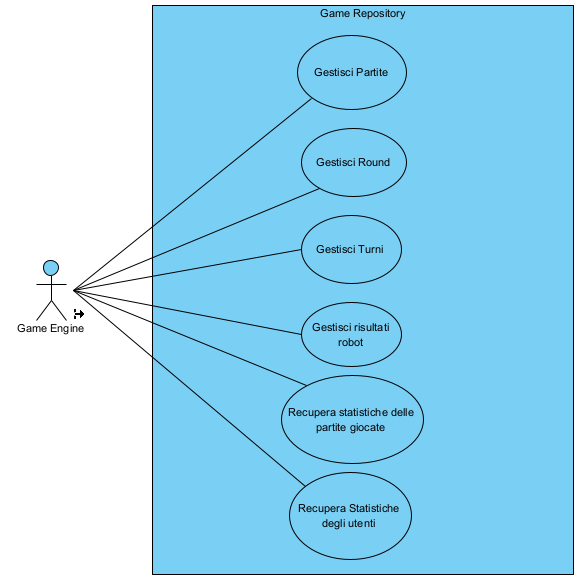
\includegraphics[width=0.7\textwidth]{images/2Analisi Requisiti/usecase.png}
    \caption{Casi d'uso}
    \label{fig:usecase}
\end{figure}


\subsection{Attori}
In questa sezione, sono descritti gli attori individuati durante l'analisi dei requisiti. Gli attori presentati saranno poi indicati anche come \textbf{utenti} del sistema.
\paragraph{Game Engine}
Il \textit{Game Engine} è l'utente utilizzatore del servizio che si occupa di implementare le logiche di gioco. Questo utente garantisce che tutti i dati salvati all'interno del \textit{Game Repository} siano coerenti.

\subsection{Requisiti Funzionali}

In questa sezione, saranno analizzati i casi d'uso per ricavarne dei requisiti funzionali. In particolare, per ogni caso d'uso sarà fornita una storia utente e un tabella riassuntiva.

\subsubsection{Gestione delle partite}
Una partita (o \textit{game}) è formata da \textit{round} durante ciascuno dei quali ogni giocatore gioca un turno. In particolare, ogni turno prevede l'esecuzione dei test generati e la registrazione dei risultati nel \textit{Game Repository}.
Una  \gls{game} può seguire diversi scenari che indicano le modalità con cui viene svolta (regole, giocatori). Questo caso d'uso genera i seguenti requisiti:
\begin{itemize}
    \item Creazione partita: quando viene creata la partita, il \textit{Game Repository} registra i partecipanti e lo scenario identificato e crea i round che saranno giocati;
    \item Cancellazione partita: una partita può essere cancellata insieme a tutti i dati associati ad essa;
    \item Modifica partita: l'utente può aggiornare lo stato della partita mantenendo l'integrità dei dati;
    \item Ricerca partita: l'utente può recuperare le informazioni essenziali di una partita a partire dalle quali può ricostruire tutti i round giocati;
    \item Recupero partite: l'utente, specificando eventualmente dei filtri, può recuperare le partite;
\end{itemize}

\begin{table}[H]
  \center
  \begin{tabular}{|l|c|p{0.5\linewidth}|}
    \hline
    ID & Nome & Descrizione \\
    \hline
        G-01 & Creazione partita  & Da utente, si vuole creare una partita specificando i giocatori partecipanti, lo scenario (ovvero, numero di turni, numero di giocatori umani e robot) e la classe da testare. \\
        \hline
        G-02 & Cancellazione partita  & Da utente, si vuole cancellare una partita e tutti i dati associati ad essa. \\
        \hline
        G-03 & Modifica partita  & Da utente, si vuole modificare una partita in corso senza compromettere l'integrità della stessa. \\
        \hline
        G-04 & Recupero partita  & Da utente, si vuole recuperare lo stato di una partita con la possibilità di esplorare i round e i turni di ciascun \gls{player} \\
        \hline
        G-05 & Recupero partite  & Da utente, si vogliono recuperare le partite applicando dei filtri (ad esempio prendere solo quelle appartenenti ad un intervallo temporale). \\
    \hline
  \end{tabular}
  \caption{Gestione partite: requisiti funzionali}
  \label{tab:0x_functional_requirements}
\end{table}


\subsubsection{Gestione dei round}
In ogni \gls{round}, ogni giocatore gioca un \gls{turn} in cui genera delle classi che risolvono il problema assegnato. In base all'esito del test al giocatore è assegnato un punteggio che dovrà essere salvato nel turno dello stesso. In particolare, ogni round avrà uno e un solo vincitore che sarà deciso dall'utente. Questo caso d'uso genera i seguenti requisiti:

\begin{itemize}
    \item Creazione round: quando viene creata la partita, il \textit{Game Repository} predispone i
    round da giocare , associando le classi da testare ad ogni round;
    \item Cancellazione round: un round può essere cancellato dal sistema insieme a tutti i turni associati;
    \item Modifica round: un round può essere aggiornato dall'utente per modificarne la durata o assegnare il vincitore;
    \item Ricerca round: l'utente può recuperare lo stato di un round insieme a tutti tutti effettuati dai giocatori;
    \item Recupero round: l'utente può recuperare tutti i round di una partita;
\end{itemize}

\begin{table}[H]
  \center
  \begin{tabular}{|l|c|p{0.5\linewidth}|}
    \hline
    ID & Nome & Descrizione \\
    \hline
        G-11 & Creazione round  & Da utente, si vuole suddividere la partita in round durante il quale ogni giocatore eseguirà il proprio turno. \\
        \hline
        G-12 & Cancellazione round & Da utente, si vuole cancellare un round e tutti i dati degli utenti associati, mantenendo l'integrità dei dati. \\
        \hline
        G-13 & Modifica round  & Da utente, si vuole aggiornare lo stato di round modificando impostazioni sulle regole o assegnando un vincitore. \\
        \hline
        G-14 & Recupero round  & Da utente, si vuole recuperare un round con le informazioni relative ai turni giocati. \\
        \hline
        G-15 & Recupero round  & Da utente, si vogliono recuperare tutti i round di una determinata partita. \\
    \hline
  \end{tabular}
  \caption{Gestione round: requisiti funzionali}
  \label{tab:1x_functional_requirements}
\end{table}


\subsubsection{Gestione turni}
In ogni turno, un giocatore genera delle classi di test che vengono eseguite dal sistema di testing che genera un punteggio. Il \textit{Game Repository} deve salvare i file prodotti dal giocatore e i punteggi assegnati. Inoltre, l'utente può cancellare o modificare il turno di un giocatore. I requisiti generati sono i seguenti:
\begin{itemize}
    \item Creazione turno: quando un giocatore sottomette la sua risposta, il sistema salva i file prodotti insieme ai punteggi assegnati;
    \item Cancellazione turno: l'utente può cancellare il turno di un giocatore;
    \item Modifica turno: l'utente può modificare il turno di un giocatore;
    \item Ricerca turno: l'utente può effettuare la ricerca di un turno di un giocatore al fine di ottenere classi generate e punteggi ottenuti;
    \item Recupero turni: l'utente può recuperare il dettaglio dei turni di un particolare round;
\end{itemize}

\begin{table}[H]
  \center
  \begin{tabular}{|l|c|p{0.6\linewidth}|}
    \hline
    ID & Nome & Descrizione \\
    \hline
        G-21 & Creazione turno  & Da utente, si vogliono salvare i file di un giocatore e i relativi punteggi ottenuti da un esecuzione dei test. \\
        \hline
        G-22 & Cancellazione turno & Da utente, si vuole cancellare il turno di un giocatore. \\
        \hline
        G-23 & Modifica turno  & Da utente, si vuole aggiornare lo stato di un turno di un giocatore effettuando delle modifiche alle classi generate o ai punteggi ottenuti. \\
        \hline
        G-24 & Recupero turno  & Da utente, si vuole recuperare lo stato di un turno di un giocatore inclusi i file creati. \\
        \hline
        G-25 & Recupero turni  & Da utente, si vogliono recuperare tutte le informazioni dei turni di un round. \\
    \hline
  \end{tabular}
  \caption{Gestione turni: requisiti funzionali}
  \label{tab:2x_functional_requirements}
\end{table}


\subsubsection{Gestione risultati dei Robot}
Per ogni classe da testare, o "livello" di una partita, è necessario confrontare i risultati dei giocatori con quelli dei robot, che consistono negli strumenti di testing automatico Randoop e EVOsuite. Piuttosto che calcolare i risultati dei robot durante ogni partita, si è scelto di memorizzarli una volta all'atto della creazione del livello, per poi recuperarli in un secondo momento. Il \textit{Game Repository} deve quindi salvare i punteggi dei robot per ogni classe da testare, potendo distinguere tra i due tipi di tool automatici e associando a ogni risultato un livello di difficoltà.
I requisiti generati sono i seguenti:
\begin{itemize}
    \item Creazione risultati robot: l'utente crea i risultati dei robot specificando la classe testata, il tipo di robot, la difficoltà e i punteggi;
    \item Cancellazione risultati robot: l'utente può cancellare i risultati di un robot specificando la classe da testare;
    \item Ricerca risultati robot: l'utente può effettuare la ricerca di un particolare tipo di robot al fine di ottenere i punteggi relativi a una classe da testare per una specifica difficoltà;
\end{itemize}

\begin{table}[H]
  \center
  \begin{tabular}{|l|c|p{0.5\linewidth}|}
    \hline
    ID & Nome & Descrizione \\
    \hline
        G-31 & Creazione risultati robot  & Da utente, si vogliono salvare i punteggi di diversi tipi di robot, ottenuti dall'esecuzione dei test, registrando il livello di difficoltà. \\
        \hline
        G-32 & Cancellazione risultati robot & Da utente, si vuole cancellare i punteggi di un robot per una specifica classe testata. \\
        \hline
        G-33 & Ricerca risultati robot & Da utente, si vuole recuperare i punteggi ottenuti da un robot relativi ad una specifica classe e difficoltà. \\
    \hline
  \end{tabular}
  \caption{Gestione turni: requisiti funzionali}
  \label{tab:2x_functional_requirements}
\end{table}
\clearpage

\subsection{Requisiti Non Funzionali}


In \cref{tab:non_functional_requirements} sono mostrati i requisiti non funzionali individuati.

\begin{table}[H]
  \center
  \begin{tabular}{|l|c|p{0.5\linewidth}|}
    \hline
        ID & Nome & Descrizione \\
        \hline
        NFR-01 & Gestione dei file dei giocatori  & Quando viene giocato il turno, bisogna conservare i file generati dai giocatori in modo tale da rendere accettabili le \textit{performance} della base dati e da permettere le operazioni di lettura e aggiornamento. \\
        \hline
        NFR-02 & Osservabilità & Il sistema deve poter esporre contatori e metriche utili per analizzare performance ed effettuare attività di ottimizzazione.\\ 
        \hline
        NFR-03 & Compliance & Il sistema deve esporre un'interfaccia che implementa lo standard Open API in quanto sarà utilizzato da altri servizi.\\
        \hline
        NFR-04 & Paginazione & Quando vengono recuperate più partite, round o turni devono essere previsti dei meccanismi di paginazione che si occupano di limitare la quantità dei dati letta e trasmessa.\\
        \hline
        NFR-05 & Sicurezza & Ogni richiesta che arriva al sistema deve essere autenticata. Nell'ambito specifico di questo progetto, l'autenticazione è gestita da un altro servizio.\\
        \hline
    \hline
  \end{tabular}
  \caption{Requisiti non funzionali}
  \label{tab:non_functional_requirements}
\end{table}

\clearpage

\section{Progettazione}
\subsection{Architettura generale del progetto}
Fissati i requisiti, si è scelto di analizzare il problema con un approccio ispirato a \textbf{Domain Driven Design} in cui si è cercato di progettare le funzionalità dal punto di vista delle entità del sistema. Questa strategia mira a dividere l'architettura iniziale in componenti indipendenti.\\
In particolare, a valle delle iterazioni, l'architettura iniziale è stata raffinata nel corso delle lezioni fino ad arrivare a quella mostrata in \cref{fig:context}:

\begin{figure}[H]
    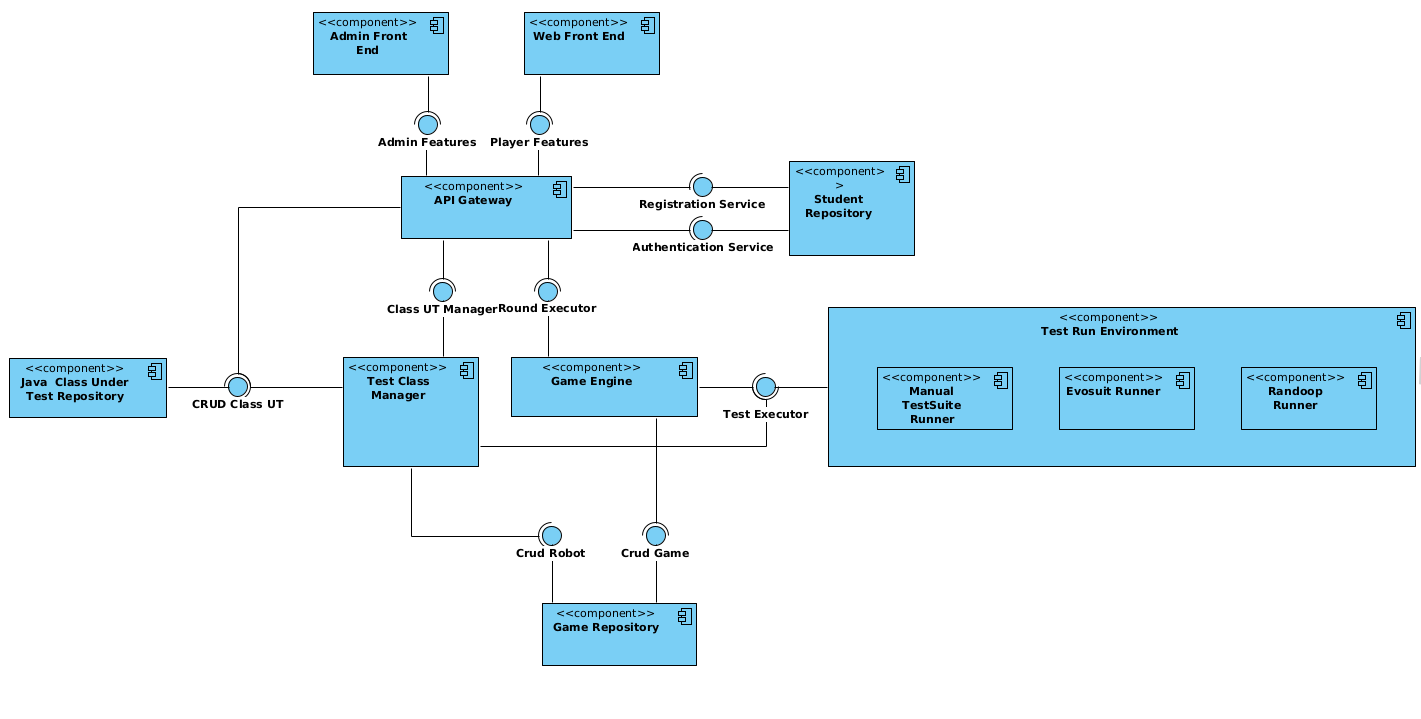
\includegraphics[width=\textwidth]{images/3Progettazione/context.png}
    \caption{Context diagram}
    \label{fig:context}
\end{figure}

L'architettura mostrata è di tipo \textit{frontend}-\textit{backend}. In particolare, sono stati previsti due tipi di \textit{frontend} (uno per i giocatori e un altro per l'amministratore). Entrambi, si interfacciano con il componente API gateway che si occupa di indirizzare le richieste ai servizi giusti e di effettuare le operazioni di autenticazione e autorizzazione. Questo componente rappresenta l'unico punto di contatto tra i \textit{frontend} e il \textit{backend}. Di seguito sono descritti gli scenari di operatività della soluzione.

\subsubsection{Caricamento delle classi di test}
L'amministratore, attraverso il frontend dedicato carica le classi da utilizzare per le partite degli utenti. All'atto della creazione, attraverso il \textit{Test Class Manager} viene eseguito il testing per ogni livello di difficoltà del gioco interagendo con il componente \textit{Test Run Environment}. Una volta generati, i risultati dei test sono salvati nel \textit{Game Repository}; mentre le classi sono salvate nel componente \textit{Java Class Under Test}. Il processo è riassunto nel diagramma di flusso in 

\begin{figure}[H]
    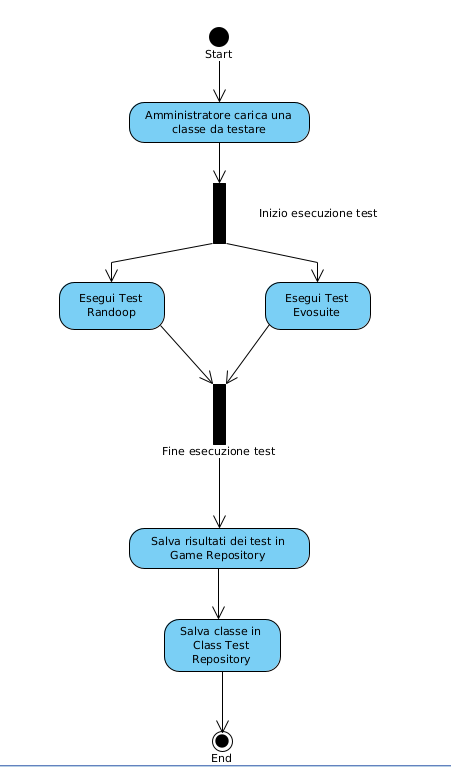
\includegraphics[width=0.7\textwidth]{images/3Progettazione/scenario_admin.png}
    \caption{Flusso caricamento classe dall'amministratore}
    \label{fig:admin_scenario}
\end{figure}

\subsubsection{Scenario di gioco}
Un giocatore, attraverso il proprio frontend, decide di partecipare ad una partita tra quelle esistenti o, eventualmente, ne può creare una da zero. Ogni partita è composta da Round, con robot da sfidare che svolgono le proprie mosse (turni) in ogni round fino alla fine della stessa. Infine, il \textit{Game Engine} decreterà un vincitore in base ai punteggi registrati ed eventuali altre metriche configurate.
Per i giocatori, il componente di riferimento è il \textit{Game Engine}. Esso si occupa di gestire la logica di gioco preoccupandosi di interagire con l'ambiente di testing per eseguire i dati di input degli utenti e con il \textit{game repository} che si occupa di memorizzare tutte le informazioni riguardanti le partite e i file prodotti dai giocatori. Il processo è riassunto nel diagramma di flusso in \cref{fig:flusso}.

\clearpage
\paragraph{Diagramma ER}
Di seguito è mostrato il diagramma Entità Relazione del sistema, con una breve descrizione degli attributi e delle relazioni.

\begin{figure}[H]
    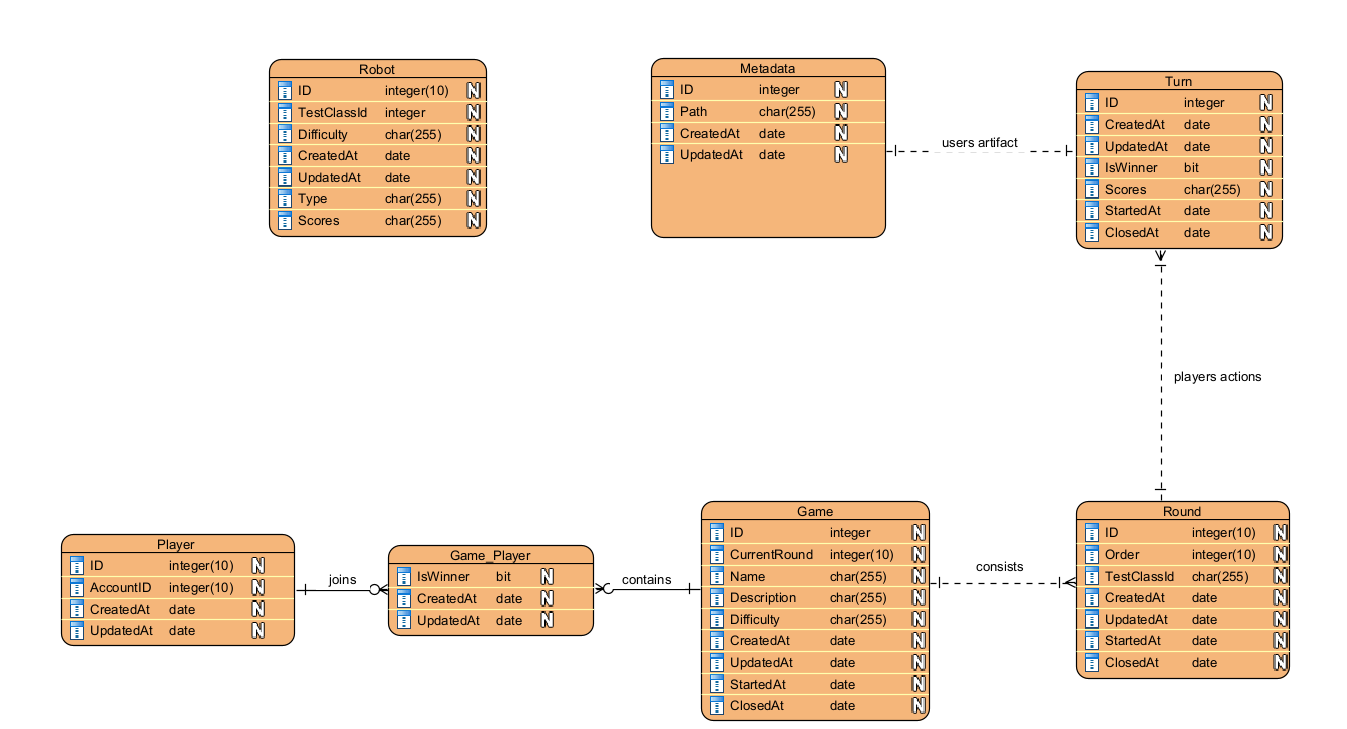
\includegraphics[width=\textwidth]{images/3Progettazione/er.png}
    \caption{Diagramma ER}
    \label{fig:er}
\end{figure}

Prima di analizzare gli attributi specifici di ogni entità è da notare che tutte possiedono i seguenti campi, utilizzati per tracciare la data di creazione e modifica:
\begin{itemize}
    \item \textbf{CreatedAt}
    \item \textbf{UpdatedAt}
\end{itemize}
Le entità di cui si deve tracciare lo stato di apertura e chiusura posseggono inoltre i seguenti attributi:
\begin{itemize}
    \item \textbf{StartedAt}
    \item \textbf{ClosedAt}
\end{itemize}

Di seguito la descrizione degli attributi divisi per entità.

\paragraph{Game}
\begin{itemize}
    \item \textbf{ID}: identificativo univoco
    \item \textbf{Current Round}: indica il numero del round corrente
    \item \textbf{Name}: nome della partita
    \item \textbf{Description}: descrizione della partita
    \item \textbf{Difficulty}: grado di difficoltà della partita
\end{itemize}

\paragraph{Player}
\begin{itemize}
    \item \textbf{ID}: identificativo univoco
    \item \textbf{AccountID}: identificativo fornito dal componente Student Repository, che contiene i dati relativi ai giocatori
\end{itemize}

\paragraph{Game\_Player}

\begin{itemize}
    \item \textbf{IsWinner}: valore booleano che indica il vincitore finale della partita
\end{itemize}

\paragraph{Round}
\begin{itemize}
    \item \textbf{ID}: identificativo univoco
    \item \textbf{Order}: indica l'ordine dei round all'interno della partita (primo round, secondo ,etc.)
    \item \textbf{TestClassId}: Identificativo della classe da testare presente presente nel Class UT Repository
\end{itemize}

\paragraph{Turn}
\begin{itemize}
    \item \textbf{ID}: identificativo univoco
    \item \textbf{IsWinner}: valore booleano che indica il vincitore del singolo round
    \item \textbf{Scores}: i punteggi relativi al giocatore che ha completato un round, calcolati dal componente di testing e compilazione.
\end{itemize}


\paragraph{Metadata}
\begin{itemize}
    \item \textbf{ID}: identificativo univoco
    \item \textbf{Path}: il percorso relativo nel file system in cui sono memorizzati i file delle classi testate dall'utente.
\end{itemize}

\subsection{Architettura Game Repository}
L'architettura del componente è ispirata al modello \textbf{Domain Driven Design} (DDD) \cite{hippchen2017designing} in cui ogni entità risulta indipendente dalle altre. Come mostrato in \cref{fig:arch}, ogni elemento logico dell'applicazione (individuato nel diagramma in \cref{fig:er}), ha a sua disposizione un \textit{Controller} che utilizza un \textit{Service}. Questi due componenti (realizzati per ogni entità) interagiscono con un ORM che implementa lo schema relazionale sul database.\\

Si noti che le fasce orizzontali rosa sono tra loro indipendenti e che l'implementazione delle classi \textit{Service} sono astratte da un'interfaccia. Questa scelta, non solo garantisce un basso accoppiamento tra le entità, ma ne favorisce anche la testabilità in quanto fornendo un'implementazione \textit{mock} del service è possibile testare indipendentemente le classi \textit{Controller} e \textit{Service}. 
\begin{figure}
    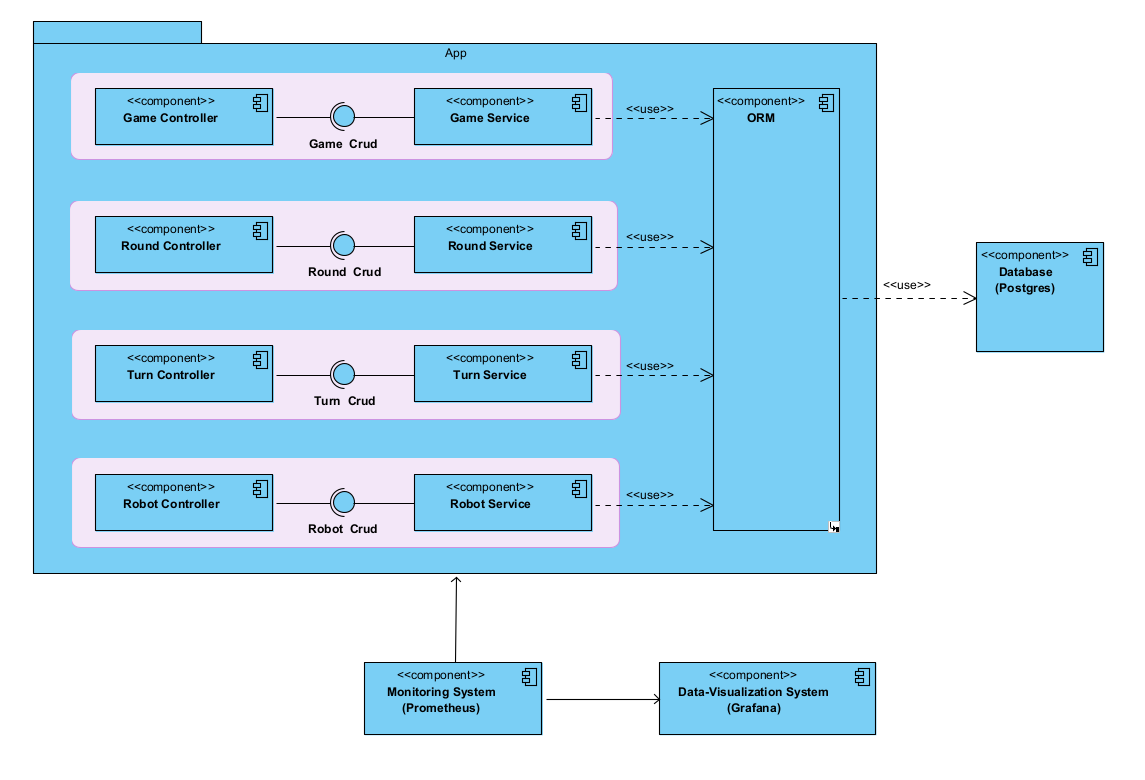
\includegraphics[width=\textwidth]{images/3Progettazione/architettura.png}
    \caption{Architettura Game Repository}
    \label{fig:arch}
\end{figure}

Lo stile Domain Driven è un'estensione concettuale di quello esagonale\cite{hippchen2017designing} e può essere utilizzato per implementare microservizi secondo il principio \textbf{SOLID}. \\

I domini applicativi rappresentati in \cref{fig:arch} sono stati raffinati nel System Domain Model \cref{fig:sdm}. Si noti che ciascuna entità (in verde) implementa sia il pattern DTO \cref{s:dto} che Dependency Injection \cref{s:di} e che inoltre, sono tra loro indipendenti; invece le relazioni della base dati sono rappresentate nel package \textit{Model} (in rosa).

\begin{figure}
    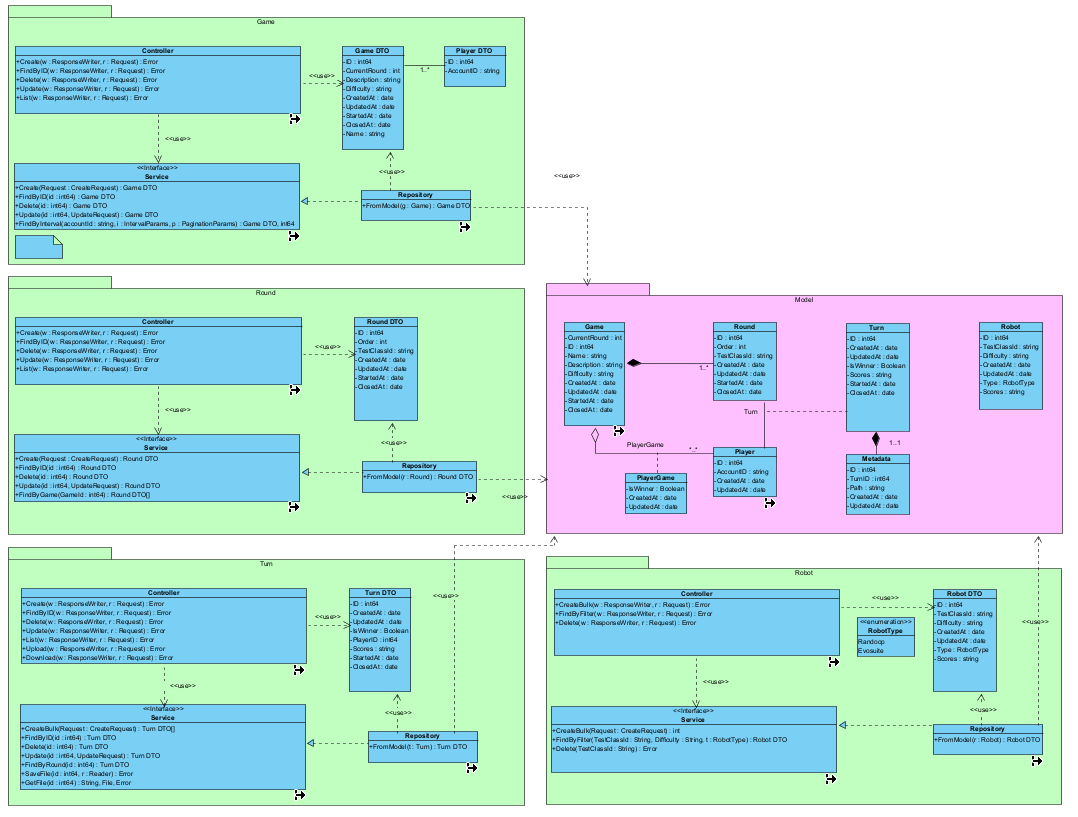
\includegraphics[width=\textwidth]{images/3Progettazione/sdm.png}
    \caption{System Domain Model}
    \label{fig:sdm}
\end{figure}


\clearpage

\subsection{Pattern utilizzati}
\subsubsection{Pattern: Facade}
Il pattern Facade viene utilizzando quando una classe \textit{Client} deve interagire con altri componenti per realizzare una funzionalità complessa (\cref{fig:facade1}). La soluzione a questo problema consiste nel creare una classe proxy \textit{Facade} che nasconde la complessità dell'operazione esponendo un solo metodo chiaro, abbassando il grado di accoppiamento della classe \textit{Client} con quelle che forniscono servizi (\cref{fig:facade2}).

\begin{figure}[H]
    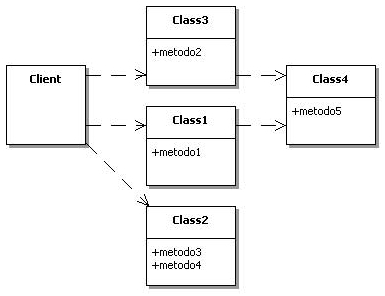
\includegraphics[width=0.5\textwidth]{images/3Progettazione/facade1.png}
    \caption{Situazione generica in cui è possibile utilizzare il pattern \textit{Facade}}
    \label{fig:facade1}
\end{figure}


\begin{figure}[H]
    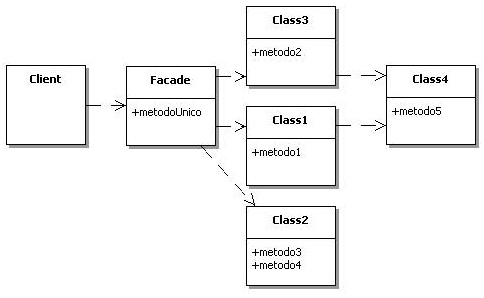
\includegraphics[width=0.5\textwidth]{images/3Progettazione/facade2.png}
    \caption{Applicazione del pattern \textit{Facade} al problema in \cref{fig:facade1}}
    \label{fig:facade2}
\end{figure}

All'interno del componente progettato, il pattern \textit{Facade} è stato utilizzato per semplificare la gestione degli accessi ai risultati dei robot, in quanto, dovendo gestire la moltitudine di risultati prodotti da \textit{Randoop}, è opportuno semplificare sia l'operazione di scrittura (accettando in ingresso più valori per singolo robot), ma anche in lettura tornando un valore random nel caso in cui si decida di prelevare un risultato specifico.

\subsubsection{Pattern: Dependency Injection} \label{s:di}
Il pattern \textbf{Dependency Injection} (DI) è utilizzato per ridurre l'accoppiamento tra due oggetti nel caso in cui siano legati da una relazione di tipo \textit{use}. In particolare, l'oggetto utilizzatore accetterà un'interfaccia della dipendenza grazie alla quale sono astratte le funzionalità utilizzate rendendolo, di fatto, indipendente dall'implementazione offerta.\\

All'interno del componente sviluppato tutti i \textbf{controller} accettano un'interfaccia di tipo \textit{Service} che astrae la logica implementativa che fa uso di un database per la gestione dei dati rendendo molto più semplice il testing. Infatti, in fase di test di unità, al componente controller viene fornita un'implementazione finta del servizio consentendo di testare in maniera indipendente le funzionalità di \textit{boundary} da quelle della logica applicativa.

\subsubsection{Pattern: Data Transfer Object} \label{s:dto}
Il pattern Data Transfer Object (DTO)\cite{dto} consente di creare viste personalizzate sui dati da mostrare agli utenti. Inoltre, consente di assemblare in un'unica entità oggetti appartenenti a classi diverse (\cref{fig:dto}).


\begin{figure}[H]
    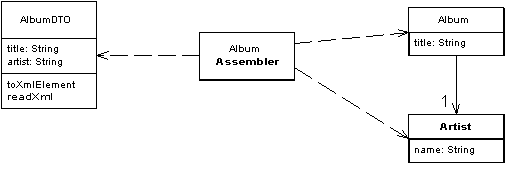
\includegraphics[width=0.8\textwidth]{images/3Progettazione/dto.png}
    \caption{Esempio di applicazione del pattern DTO}
    \label{fig:dto}
\end{figure}


All'interno del componente sviluppato, tutte le entità del modello dei dati hanno un corrispondente DTO che viene assemblato grazie alla funzione \textit{fromModel}. L'utilizzo di questo pattern conferisce all'architettura del sistema flessibilità in quanto è possibile sempre cambiare e/o modificare i dati inviati e ricevuti dai sistemi con cui ci si interfaccia senza cambiare il modello relazionale iniziale. In questo modo, si sta, di fatto, definendo un'interfaccia di I/O tra il sistema e gli altri componenti della soluzione globale.


\subsubsection{Pattern: Middleware}\label{s:middleware}
Il pattern \textbf{Middleware} consente di implementare una catena di responsabilità secondo la quale ad ogni richiesta (o messaggio) possono essere applicate diverse funzioni ed offre la possibilità di estendere le funzionalità di un'applicazione semplicemente applicando delle configurazioni (\cref{fig:middleware}).

\begin{figure}[H]
    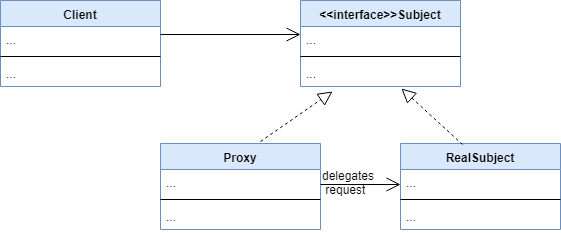
\includegraphics[width=0.8\textwidth]{images/3Progettazione/middleware.png}
    \caption{Esempio di realizzazione del pattern Middleware}
    \label{fig:middleware}
\end{figure}

All'interno dell'applicazione sviluppata il pattern \textit{middleware} è utilizato per eseguire operazioni sulla validità di richieste HTTP. Ad esempio, per richieste in scrittura sono eseguiti i seguenti middleware (illustrati in \cref{fig:mw_req}):
\begin{itemize}
    \item \textbf{rate limiting}: si controlla che un client non effettui troppe richieste ad un server;: la richiesta, una volta terminata viene mostrata sul terminale. Per ogni richiesta, sono mostrati \textit{path}, durata, metodo e codice HTTP della risposta;
    \item \textbf{controllo della validità dell'header HTTP}: una richiesta con un corpo in JSON deve necessariamente presentare l'intestazione \textit{Content-Type} con il valore di \textit{application/json};
    \item \textbf{controllo della dimensione della richiesta}: per evitare attacchi DoS o semplicemente per proteggere il database, la dimensione delle richieste è limitata da un middleware;
    \item \textbf{ip reale}: se l'applicazione risiede alle spalle di un \textit{Reverse Proxy} il valore dell'indirizzo sorgente della richiesta sarebbe sovrascritto da quello del proxy e conservato in \textit{header standard}. Questo middleware rimette l'indirizzo IP del client all'interno di quello sorgente;
     \item \textbf{autenticazione}: può essere configurato un componente che per ogni richiesta verifica se è presente un token di autenticazione e contatta un servizio esterno per verificarne la validità;
\end{itemize}

\begin{figure}[H]
    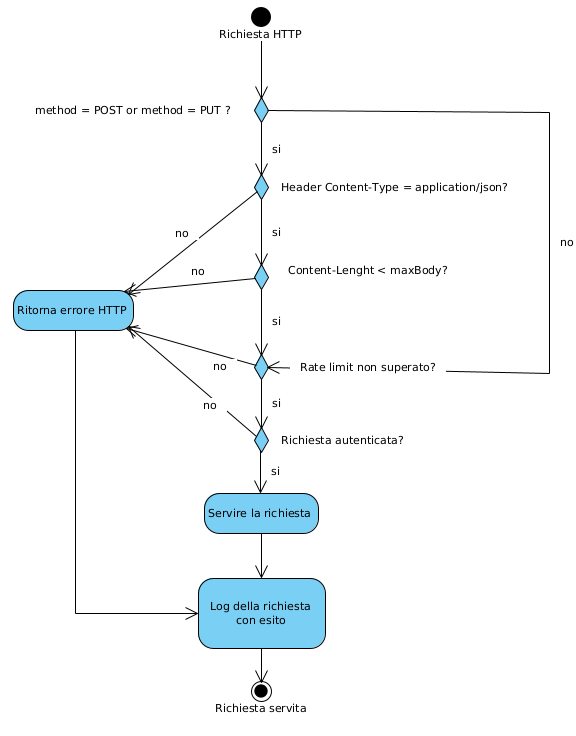
\includegraphics[width=0.8\textwidth]{images/3Progettazione/mw_req.png}
    \caption{Catena di esecuzione per una generica richiesta HTTP all'interno del componente REST Server}
    \label{fig:mw_req}
\end{figure}


Questo pattern architetturale conferisce all'applicazione la capacità di essere estesa per esempio aggiungendo un modulo di autenticazione, come mostrato in \cref{fig:mw_req}. Inoltre, attraverso un'opportuna struttura del sistema ciascun "anello" della catena può essere configurato per essere attivato o meno conferendo al sistema un alto grado di flessibilità.
\clearpage

\subsection{Tecnologie}
\subsubsection{Tecnologie analizzate}
Ai fini di implementare le funzionalità richieste sono state analizzate diverse soluzioni che prevedono l'utilizzo stack tecnologici differenti, i cui vantaggi e svantaggi sono qui elencati:

\begin{table}[H]
    \centering
    \begin{tabular}{|l|p{0.4\linewidth}|p{0.4\linewidth}|}
        \hline
         Stack & Vantaggi & Svantaggi \\
        \hline
        \hline
        Go  & 
        \begin{itemize}
          \item Performance migliori in termini di latenza per le richieste e consumo di memoria per le web application rispetto alla soluzione in Java \cite{go_java_php};
          \item GO è \textit{battery included}: non è necessaria nessuna dipendenza per essere installato,  produce un singolo file eseguibile con le dipendenze \textit{linkate} staticamente. Ciò lo rende particolarmente adatto ad uno scenario CI/CD;
          \item Possibilità di scaricare localmente le dipendenze (\textit{vendoring}) e avere un progetto sempre compilabile anche a distanza di anni;
          \item I/O asincrono e concorrenza nativamente implementata (Go routines e CSP);
          \item Linguaggio molto semplice da imparare (meno di 25 keyword) e molto stabile;
          \item Supporta nativamente strumenti per la generazione del codice automatica;
        \end{itemize} 
        & 
        \begin{itemize}
            \item Garbage collected;
            \item Poca \textit{syntactic sugar} che può rendere lo sviluppo verboso;
        \end{itemize}\\ 
        \hline
    \end{tabular}
    \caption{Vantaggi e svantaggi di uno \textit{stack} basato su Go}
    \label{tab:go_tech_stack}
\end{table}

\begin{table}[H]
    \centering
    \begin{tabular}{|l|p{0.4\linewidth}|p{0.4\linewidth}|}
        \hline
         Stack & Vantaggi & Svantaggi \\
        \hline
        Java  & 
        \begin{itemize}
          \item Springboot e Hibernate è uno degli \textit{stack} tecnologici più utilizzati e maturi;
          \item Supporto per CRUD API tramite attività di configurazione e poca scrittura di codice;
        \end{itemize} 
        & 
        \begin{itemize}
            \item Garbage collected;
            \item Performance degradate rispetto alla soluzione Go e Rust \cite{go_java_php} \cite{http_benchmark};
            \item \textit{Slow startup}: richiede un grande investimento di tempo per inizializzare un progetto che lo rende poco adatto per lo sviluppo di prototipi;
        \end{itemize}\\ 
        \hline
    \end{tabular}
    \caption{Vantaggi e svantaggi di uno \textit{stack} basato su Java}
    \label{tab:java_tech_stack}
\end{table}

\begin{table}[H]
  \center
  \begin{tabular}{|l|p{0.4\linewidth}|p{0.4\linewidth}|}
    \hline
         Stack & Vantaggi & Svantaggi \\
        \hline
        PostgREST & 
        \begin{itemize}
          \item Nessuna linea di codice viene scritta;
          \item Sfrutta appieno tutte le potenzialità di PosgreSQL;
          \item Può essere utile per effettuare ricerche con filtri avanzati;
        \end{itemize} 
        & 
        \begin{itemize}
            \item Rende impossibile passare ad un altro database causando il cosiddetto \textit{vendor locking};
            \item Diventa impossibile da utilizzare quando alle operazioni CRUD bisogna aggiungere della logica. Questa logica può essere molto complicata da implementare lato database;
            \item Richiede una conoscenza avanzata del database PostgreSQL;
        \end{itemize}\\ 
        \hline
    \hline
  \end{tabular}
  \caption{Vantaggi e svantaggi nell'utilizzo di Postgrest}
  \label{tab:postgrest_tech_stack}
\end{table}


\begin{table}[H]
    \centering
    \begin{tabular}{|l|p{0.4\textwidth}|p{0.4\linewidth}|}
        \hline
         Stack & Vantaggi & Svantaggi \\
        \hline
         Rust & 
       \begin{itemize}
           \item \textit{Memory safety} a tempo di compilazione garantita senza un \textit{garbage collector} \cite{borrow_checker};
           \item Rust offre le migliori performance sia per memoria/CPU usati che per tempo di risposta delle richieste rispetto alle altre tecnologie presentate \cite{pingora} \cite{discord_rust};
           \item Compilazione di un singolo file eseguibile adatto ad uno scenario CI/CD;
           \item Axum è basato sull'engine \textit{hyper.rs} contraddistinto da prestazioni migliori rispetto alle altre soluzioni presentate \cite{http_benchmark};
           \item Semplicità nella gestione dei progetti con Cargo \cite{cargo};
       \end{itemize} & 
       \begin{itemize}
           \item Il linguaggio può risultare complicato da apprendere;
           \item Scarso supporto per l'auto-generazione del codice data una specifica OpenAPI;
           \item Linguaggio poco conosciuto, può rallentare lo sviluppo laddove non ci fosse supporto dalla \textit{community};
           \item A causa delle ottimizzazioni e dei controlli effettuati dal compilatore le \textit{build} possono essere lente;
       \end{itemize}\\
        \hline
    \end{tabular}
    \caption{Vantaggi e svantaggi di uno \textit{stack} basato su Rust}
    \label{tab:rust_tech_stack}
\end{table}

\subsubsection{Tecnologie scelte}
La soluzione finale prevede l'utilizzo dello stack basato su GO e di un database relazionale. 
In particolare è stato scelto PostgreSQL in quanto si tratta di una soluzione completamente open source, largamente utilizzata, affidabile e altamente scalabile.
Mentre il database è utilizzato per memorizzare i dati relativi alle partite e ai punteggi, si è scelto di conservare i file java delle classi testate generate dai giocatori nel file system, salvando i metadati con il relativo path in una tabella apposita, così da ottimizzare le performance. 



Per garantire l'osservabilità del sistema si è scelto di utilizzare Prometheus, uno strumento che traccia diverse metriche relative al sistema e permette di visualizzarle in dashboard elementari. 
Per permettere una visione più avanzata delle metriche a quest'ultimo è stato collegato Grafana, che permette di creare dashboard personalizzate per poi salvarle.



\clearpage
\section{Implementazione}
\subsection{Flusso partita}
In questa sezione vengono mostrate le diverse azioni dell'utente (\textit{Game Engine}) svolte durante lo svolgimento della partita, modellate come un'\textit{activity diagram}.
Ad ognuna di queste azioni corrisponde una richiesta tramite API, il cui funzionamento è modellato nella sezione successiva. 

\begin{figure}[H]
    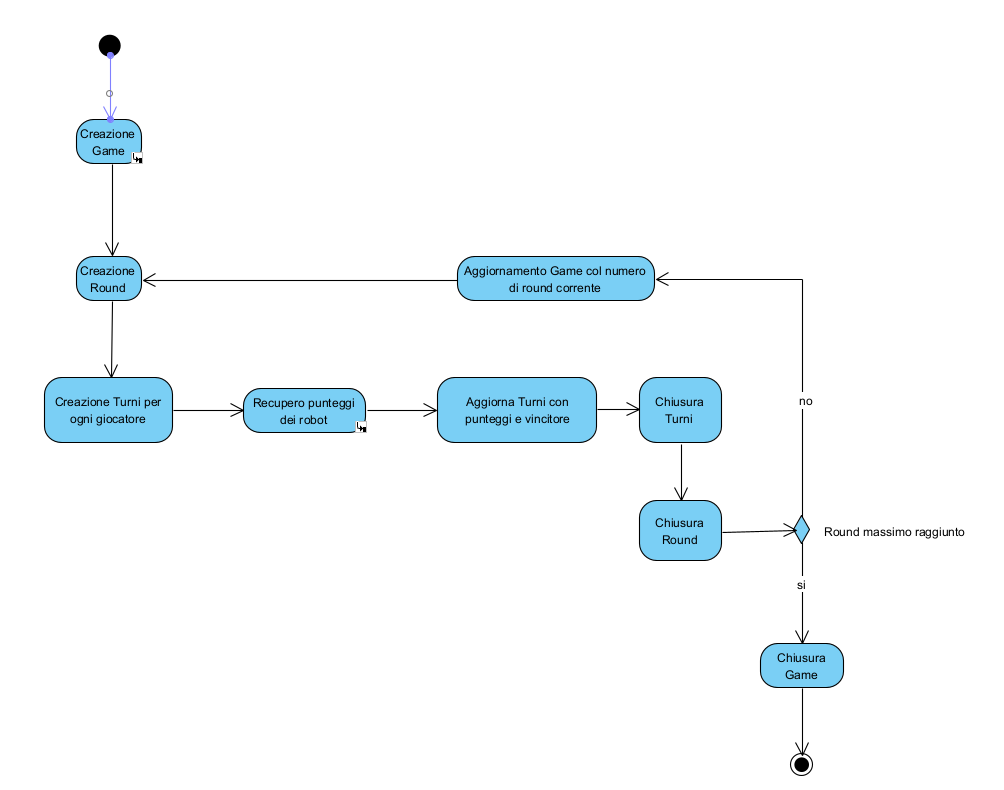
\includegraphics[width=\textwidth]{images/4Implementazione/flusso.png}
    \caption{Flusso partita}
    \label{fig:flusso}
\end{figure}

\clearpage
\subsection{Diagrammi di sequenza}
Di seguito sono modellate alcune delle richieste che l'utente  può effettuare durante lo svolgimento di una partita. 

\paragraph{Creazione Game}
Il \textit{Game Engine} invia una richiesta per la creazione della partita. Di seguito è riportato un body di esempio per la richiesta:
  \begin{lstlisting}[language=json,firstnumber=1]
{
  "name": "Game name",
  "players": [
    "id1",
    "id2"
  ],
  "description": "description",
  "difficulty": "easy"
}
    \end{lstlisting}
Nel caso in cui la richiesta non sia valida il sistema invierà un messaggio di errore, altrimenti verrà creata la partita con i relativi giocatori salvandola nel database. In seguito verrà restituito il DTO (Data Transfer Object) relativo alla partita creato dalla funzione \textit{FromModel}.

\begin{figure}[H]
    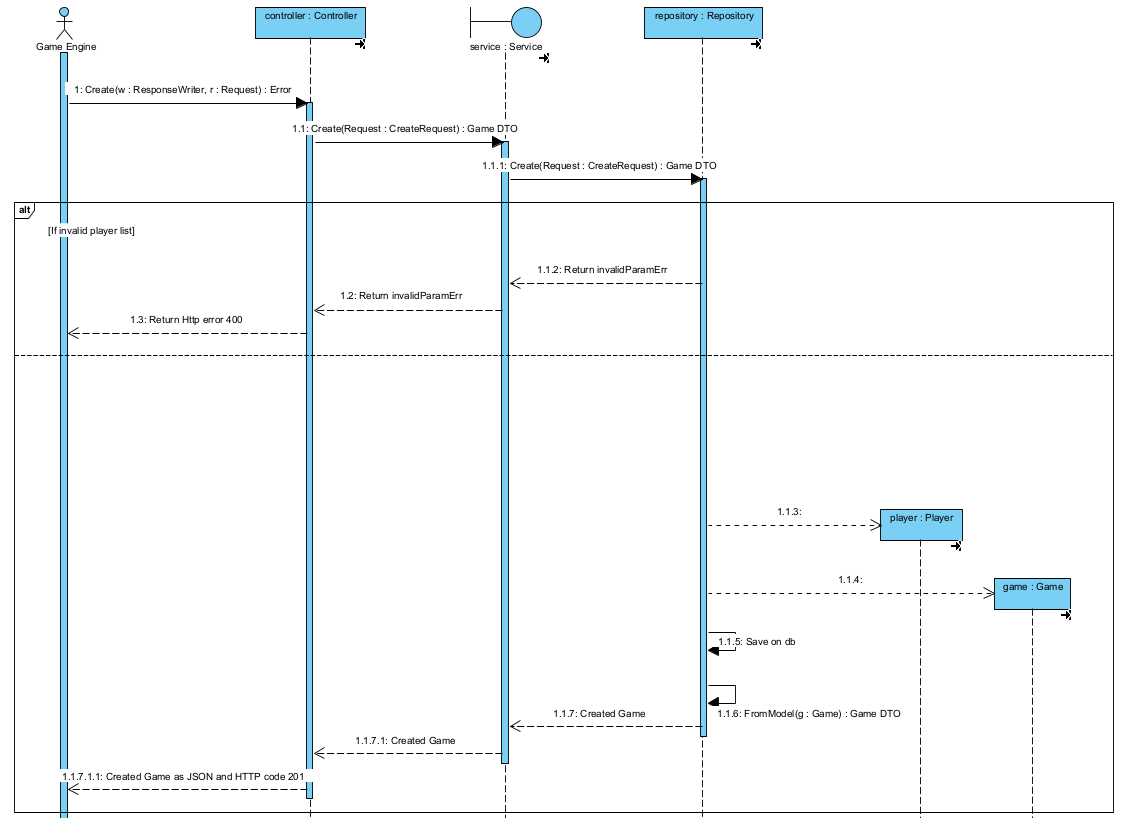
\includegraphics[width=\textwidth]{images/4Implementazione/create-game.png}
    \caption{Creazione Partita}
    \label{fig:createGame}
\end{figure}


\clearpage

\paragraph{Aggiornamento Game}
L'aggiornamento della partita è necessario qualora si volesse modificare il numero del round corrente, o indicare l'inizio e fine della partita. È possibile inoltre modificare il nome e la descrizione del game.
Il sistema controlla che la partita da modificare esista e che la richiesta abbia un body valido, dopo di che, in caso di successo, restituisce il DTO della partita modificata sotto forma di JSON.

\begin{figure}[H]
    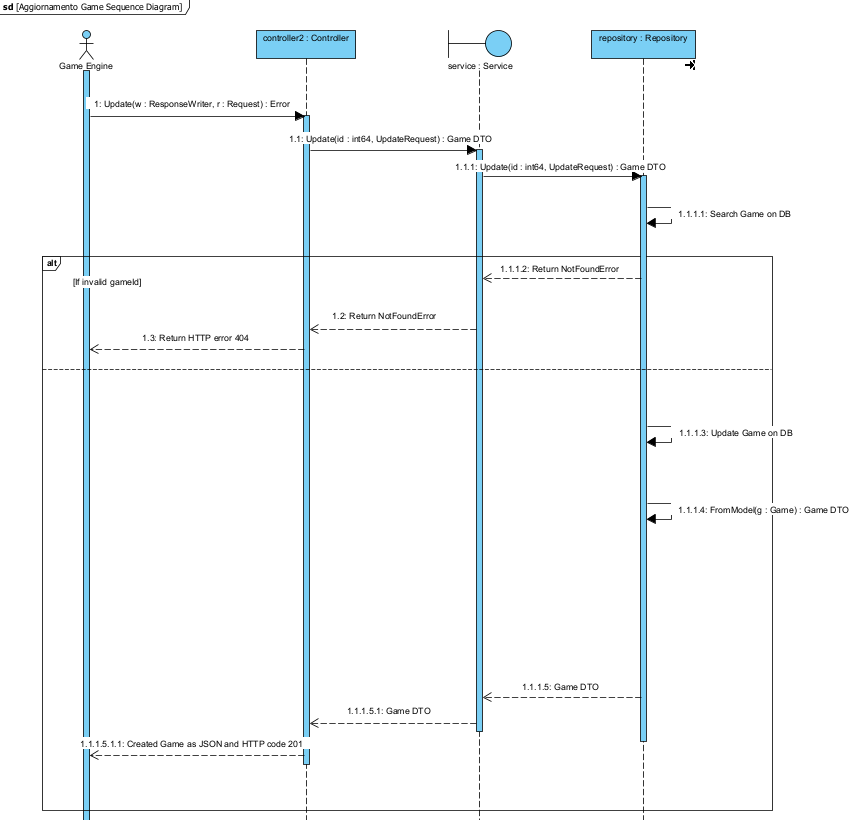
\includegraphics[width=\textwidth]{images/4Implementazione/update-game.png}
    \caption{Aggiornamento partita}
    \label{fig:updateGame}
\end{figure}

\clearpage

\paragraph{Creazione Round}
La creazione dei round avviene in maniera simile a quella delle partite. In particolare, l'utente dovrà specificare nel body della richiesta l'id del game di cui il round fa parte, e l'id della classe da testare.
Ogni round creato, oltre a un proprio id, avrà un campo chiamato \textit{order} che indicherà il suo ordine rispetto agli altri round nella partita.

\begin{figure}[H]
    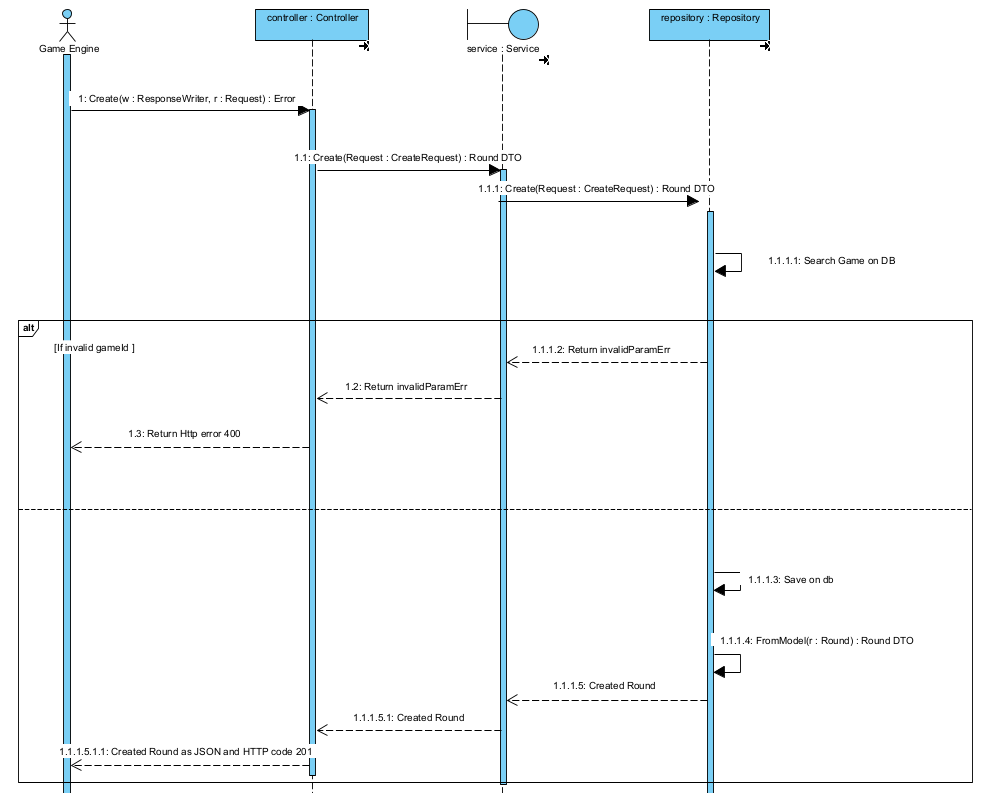
\includegraphics[width=\textwidth]{images/4Implementazione/create-round.png}
    \caption{Creazione Round}
    \label{fig:createRound}
\end{figure}

\clearpage

\paragraph{Aggiornamento Round}
L'aggiornamento del round è necessario principalmente per indicarne la data di inizio e fine.
Come nei casi precedenti il sistema controlla se la richiesta e valida e in caso di successo restituisce il DTO del round aggiornato.

\begin{figure}[H]
    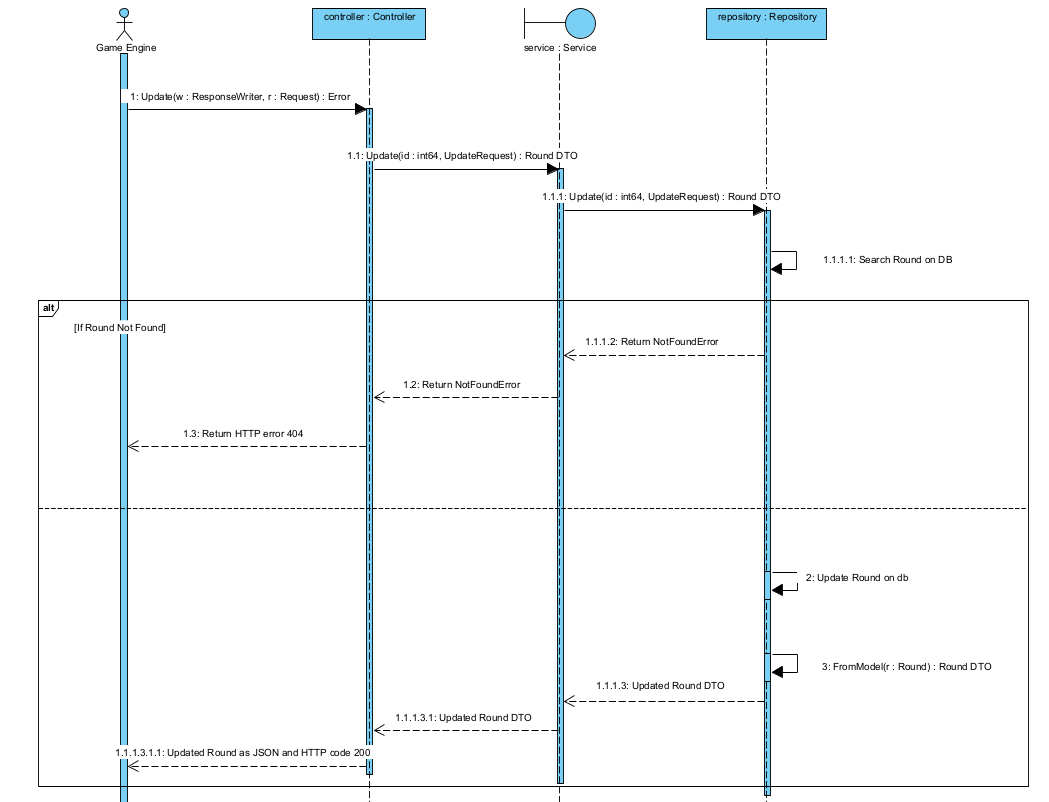
\includegraphics[width=\textwidth]{images/4Implementazione/update-round.png}
    \caption{Aggiornamento Round}
    \label{fig:updateRound}
\end{figure}

\clearpage

\paragraph{Creazione Turni}
Durante lo svolgimento di un round è necessario creare un turno per ogni giocatore. L'utente invia una richiesta contenente la lista degli id dei giocatori partecipanti e l'id del round. Nel caso sia valida, il sistema crea in loop una serie di turni associati a ogni giocatore, dove poi saranno contenuti i dati relativi alla sua prestazione , come i punteggi e l'eventuale vittoria.
Come nei casi precedenti il sistema restituisce in seguito i DTO relativi ai turni creati.

\begin{figure}[H]
    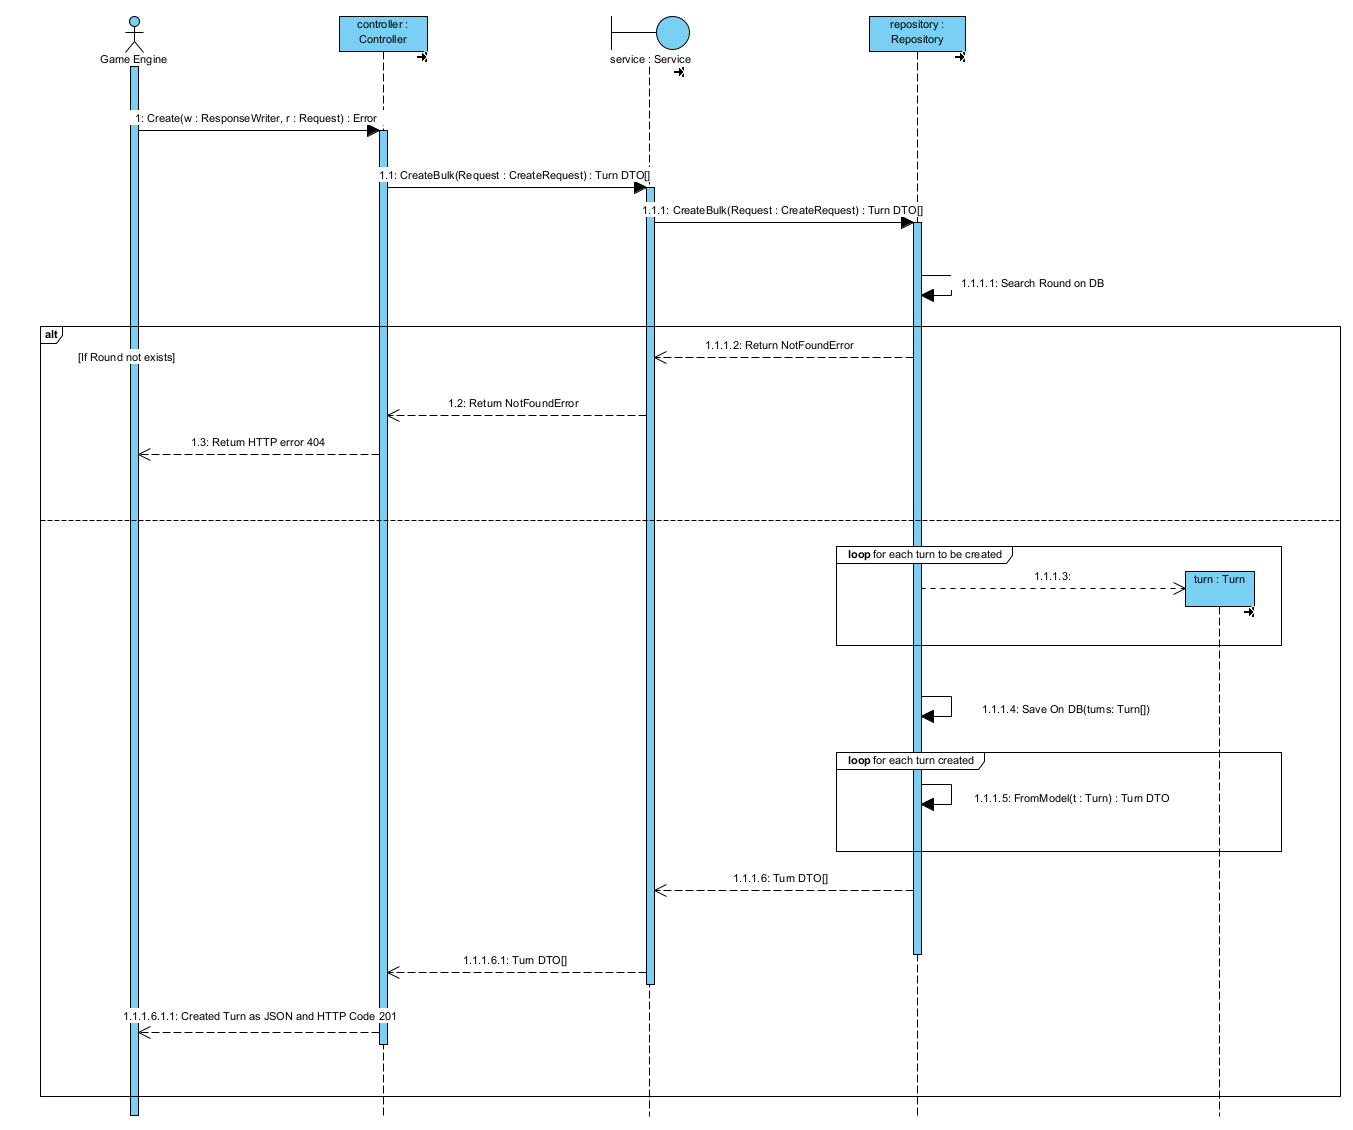
\includegraphics[width=\textwidth]{images/4Implementazione/create-turn.png}
    \caption{Creazione Turno}
    \label{fig:createTurn}
\end{figure}

\clearpage

\paragraph{Aggiornamento Turni}
L'aggiornamento dei turni è necessario nel momento in cui l'utente deve caricare i punteggi calcolati dai componenti di testing e esecuzione delle classi. Dopo aver calcolato il punteggio migliore, è inoltre possibile indicare quale degli utenti sia il vincitore del round impostando il valore \textit{isWinner} del suo round a \textit{True}.
Una volta ricevuta la richiesta il sistema controlla la sua validità e in caso positivo restituisce il DTO del turno aggiornato.

\begin{figure}[H]
    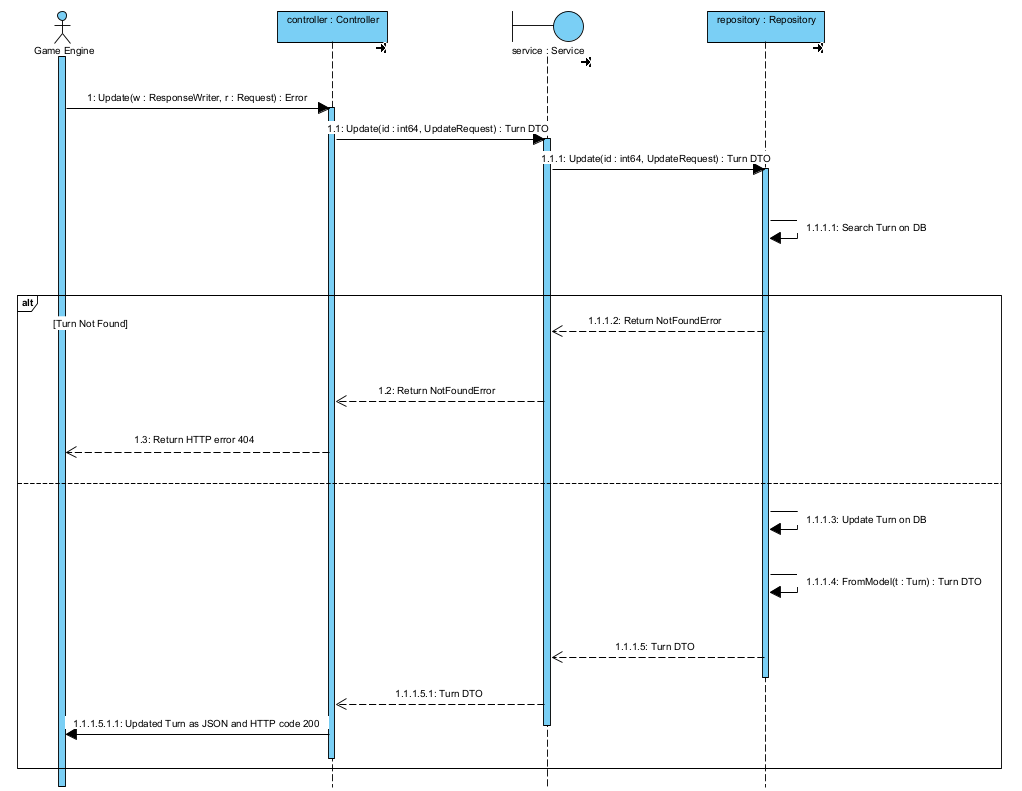
\includegraphics[width=\textwidth]{images/4Implementazione/update-turn.png}
    \caption{Aggiornamento turno}
    \label{fig:updateTurn}
\end{figure}

\clearpage

\paragraph{Recupero Punteggi Robot}
Durante ogni round l'utente dovrà recuperare i punteggi dei robot relativi alla classe di test in gioco, per paragonarli alle prestazioni dei giocatori. Nella richiesta sarà quindi necessario indicare una serie di parametri per filtrare i punteggi ottenuti:
\begin{itemize}
    \item \textit{TestClassId}: l'id della classe testata
    \item \textit{Difficulty} : la difficoltà associata ai punteggi dei robot da recuperare. È infatti possibile memorizzare diversi punteggi di un robot per la stessa classe testata classificandoli con diversi livelli di difficoltà.
    \item \textit{Type}: il tipo di robot di cui si vuole recuperare i punteggi. Fino al momento della stesura del documento sono utilizzati Randoop e EVOsuite.
\end{itemize}
Il sistema controllerà la validità della richiesta e la presenza dei punteggi cercati, e in caso di successo restituirà il DTO relativo.



\begin{figure}[H]
    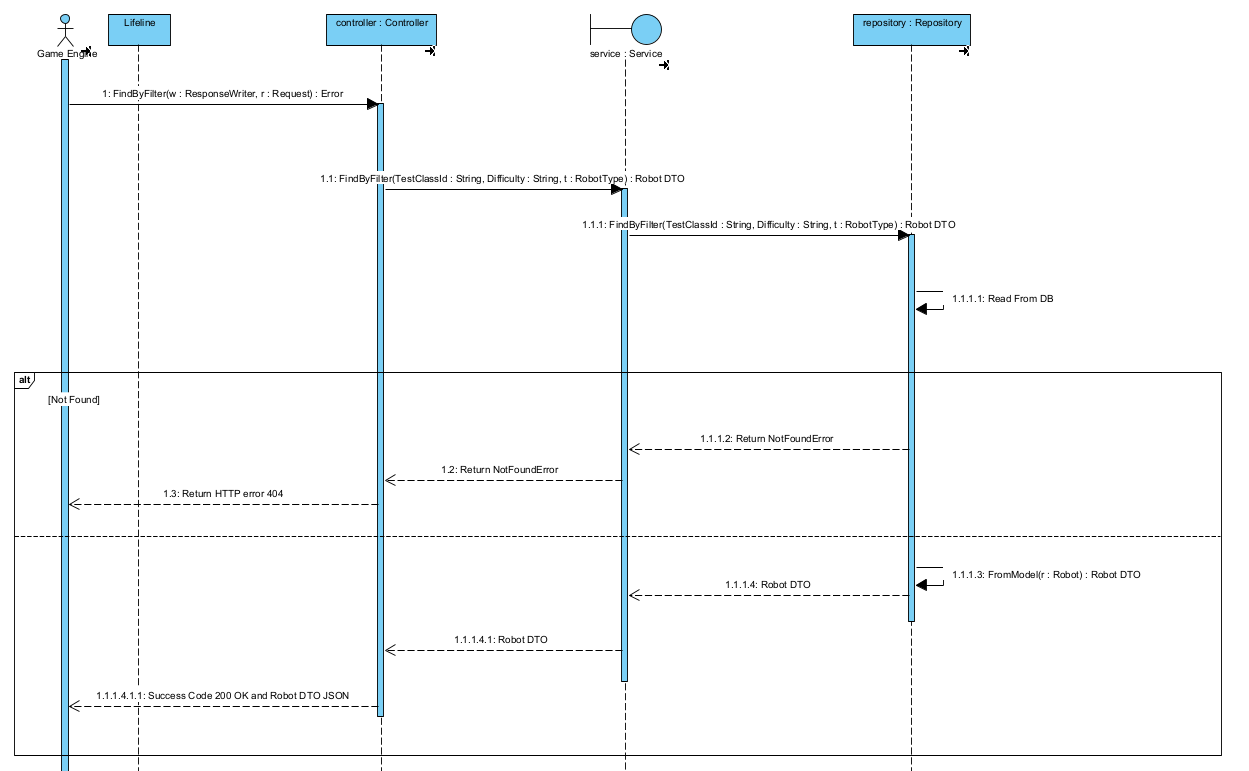
\includegraphics[width=\textwidth]{images/4Implementazione/get-robot.png}
    \caption{Recupero punteggio Robot}
    \label{fig:getRobot}
\end{figure}



\clearpage


\paragraph{Salvataggio file del turno}
A seguito della giocata di un turno da parte di uno specifico giocatore, l'utente avrà la possibilità di salvare i file prodotti contestualmente alla giocata in un unico file zip. Nella richiesta preposta sarà necessario specificare:

\begin{itemize}
    \item \textit{L'id del turno} come parametro nel path della richiesta
    \item \textit{Il File zip} come body di tipo application/zip della richiesta
\end{itemize}
Il sistema controllerà l'esistenza del turno indicato, restituendo, in caso di successo, un messaggio di avvenuto salvataggio qualora lo stesso andasse a buon fine.



\begin{figure}[H]
    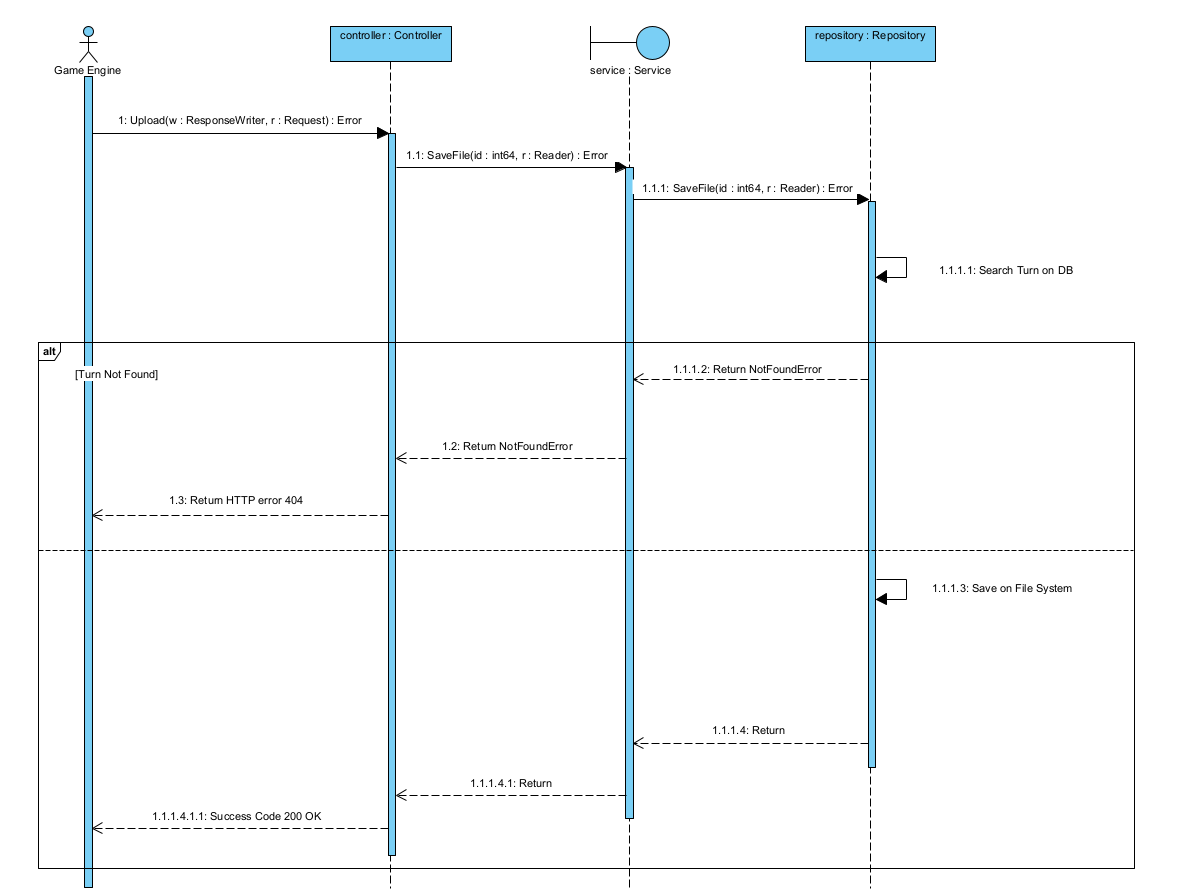
\includegraphics[width=\textwidth]{images/4Implementazione/save-file.png}
    \caption{Salvataggio file del turno}
    \label{fig:saveFile}
\end{figure}

\clearpage

\paragraph{Recupero file del turno}
L'utente potrà recuperare in qualunque momento l'archivio contenente i file associati ad uno specifico turno. Nella richiesta di recupero del file sarà necessario specificare \textit{L'id del turno}.
Il sistema controllerà l'esistenza di un file precedentemente salvato a sistema per il turno indicato, restituendo, in caso di successo, una response con Content-Type application/zip corrispondente al file zip precedentemente salvato.



\begin{figure}[H]
    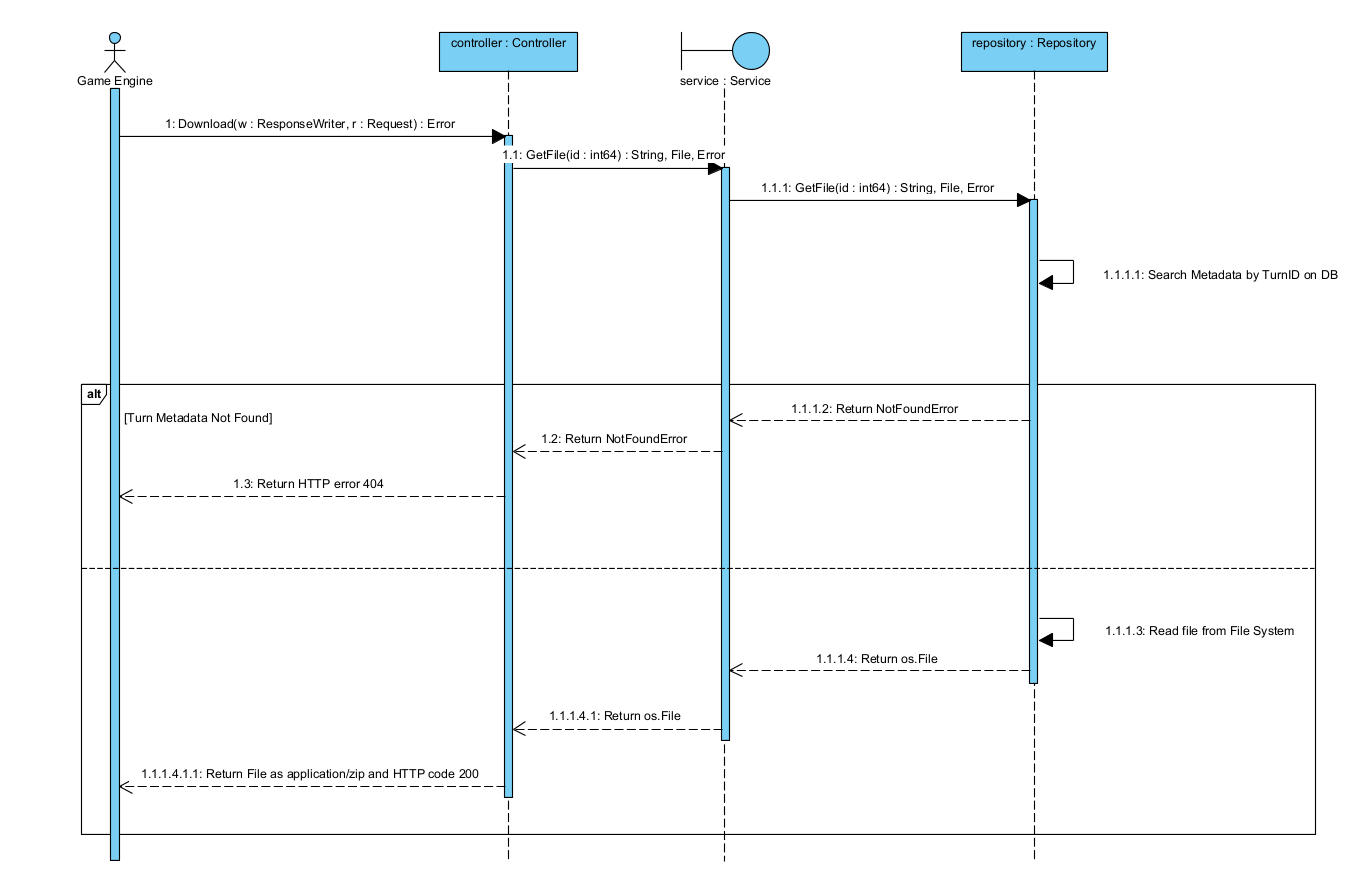
\includegraphics[width=\textwidth]{images/4Implementazione/download-file.png}
    \caption{Recupero file del turno}
    \label{fig:getFile}
\end{figure}



\clearpage


\subsection{Documentazione API}
\paragraph{Swagger}
Al fine di garantire una corretta integrazione dell'applicativo con gli altri componenti dell'architettura oggetto di altri task, si è scelto di adottare l'utilizzo di un interfaccia \textit{Swagger} che documentasse i servizi offerti dal componente realizzato.
L'interfaccia Swagger, infatti, realizza i principi della specifica \textit{OpenAPI} la quale fornisce uno standard per l'integrazione di componenti eterogenei che comunicano tramite API HTTP.
Tale interfaccia consente di presentare il dettaglio dell'API esposta dall'applicativo facilitando il testing e l'integrazione del Game Repository e fornendo informazioni relative ai singoli servizi quali path, parametri, dettaglio della request e possibili respone del servizio.
Attraverso Postman, è stata progettata la specifica OpenAPI degli endpoint ed è stata integrata attraverso github sul progetto principale. Infine, è stata effettuata un'integrazione all'interno del progetto per esporre la \textit{Swagger UI} e servire sia la specifica OpenAPI che la collection Postman quando l'applicazione viene configurata con il \textit{flag} \textbf{\textit{enableSwagger}} a \textit{True}. E possibile consultare la documentazione dell'API al link. (La stessa è riportata in \cref{fig:swagger}).

\begin{figure}[H]
    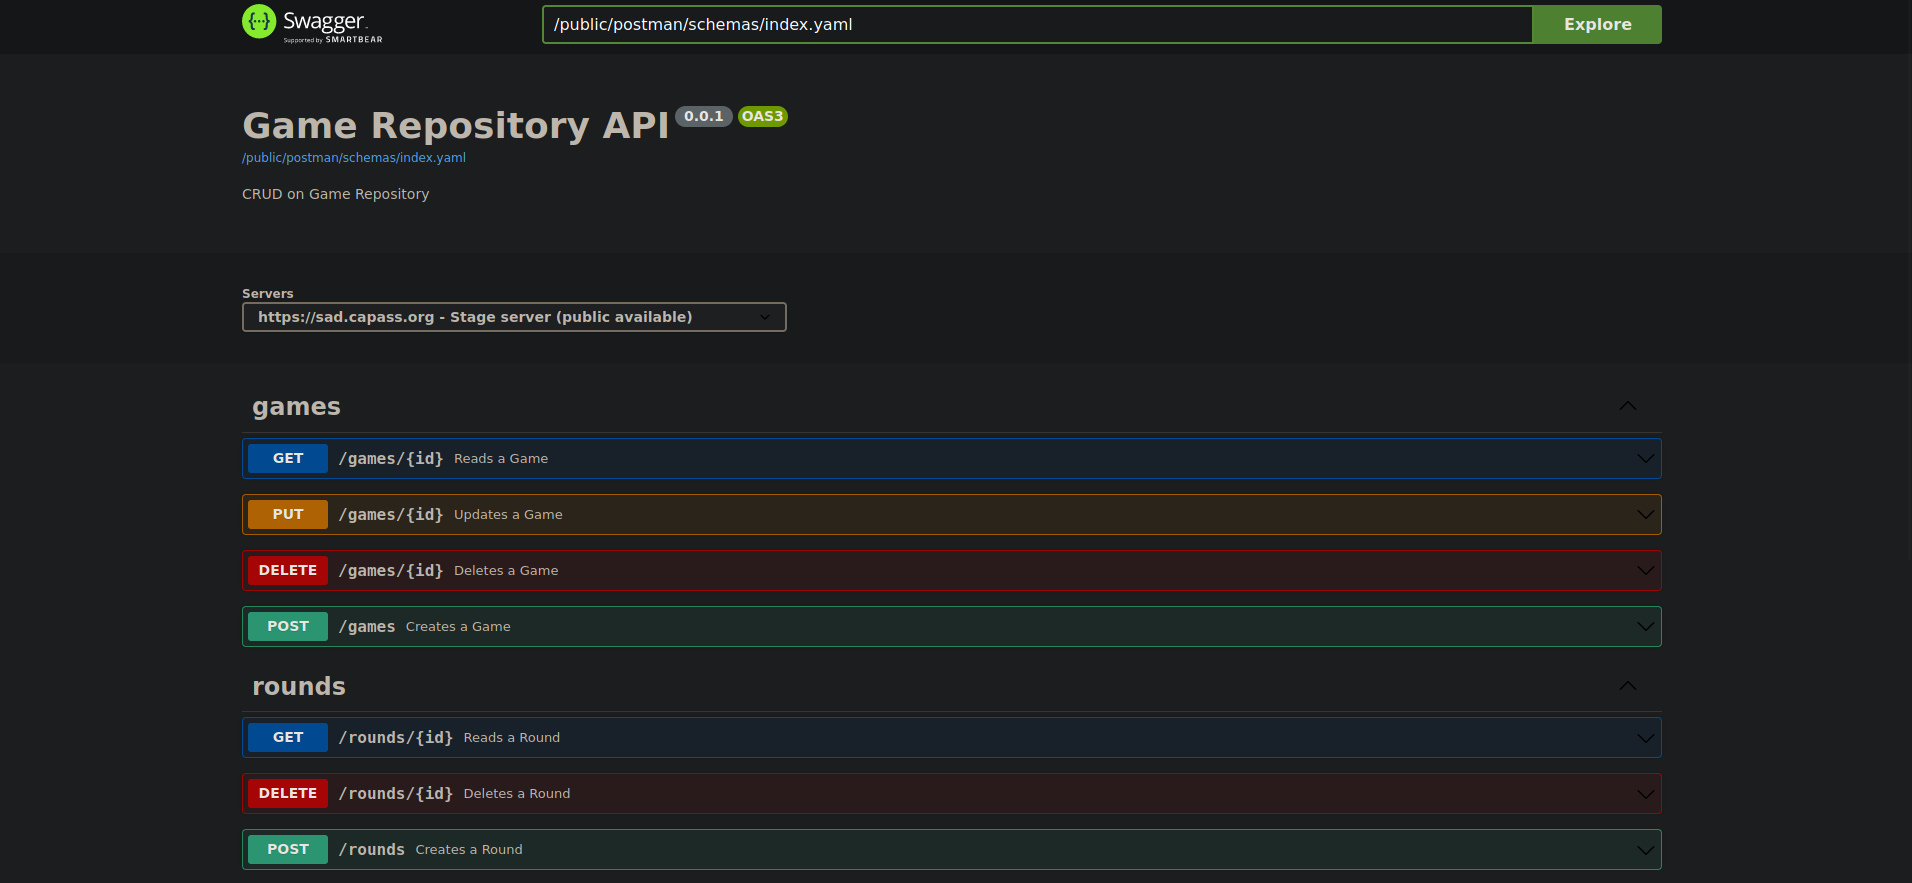
\includegraphics[width=\textwidth]{images/4Implementazione/swagger.png}
    \caption{Swagger UI}
    \label{fig:swagger}
\end{figure}

\paragraph{API Diagram}
Nei diagrammi prodotti per la documentazione dell'applicativo è incluso un Class Diagram riportante il dettaglio dei servizi esposti dall'applicativo. Visual paradigm consente infatti di modellare le API HTTP documentandone i dettagli della richiesta, i metodi, gli end-point e i possibili output.

\begin{figure}[H]
    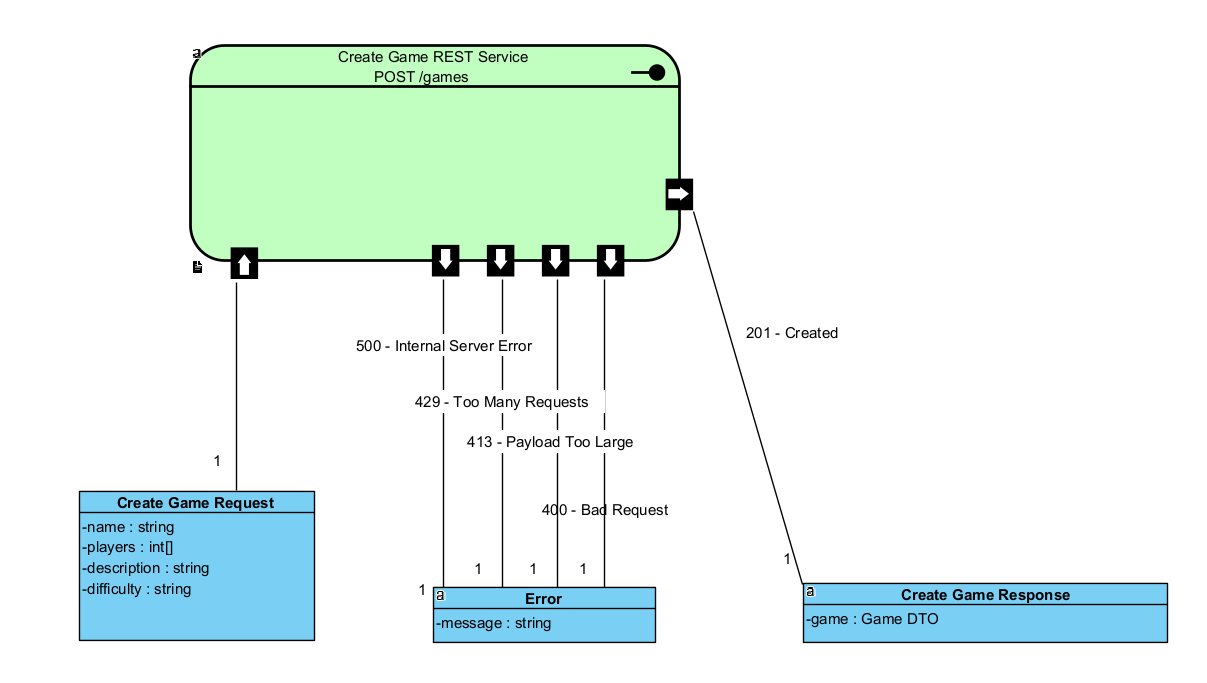
\includegraphics[width=\textwidth]{images/4Implementazione/api-class-diagram.png}
    \caption{Dettaglio del Servizio di Create Game sul diagramma delle API}
    \label{fig:apiDiag}
\end{figure}

\subsection{Prometheus \& Grafana}
Al fine di garantire l'osservabilità della soluzione si è scelto di utilizzare Prometheus e Grafana. Prometheus è un tool che offre la funzionalità di tracciare diverse metriche relative al sistema e di visualizzarle in dashboard basilari. Per estendere gli strumenti di analisi si è scelto di utilizzare Grafana, software che consente la creazione grafici e dashboard personalizzate per poi salvarle. Un esempio di dashboard è mostrato nella figura \cref{fig:grafana_dashboard}, in cui sono tracciate le seguenti metriche:
\begin{itemize}
    \item Request Rate: il numero di richieste al minuto; 
    \item CPU Usage: utilizzo in percentuale della CPU. Prometheus fornisce l'utilizzo in secondi quindi è stato calcolato come il rate in 5 minuti moltiplicandolo poi per 100;
    \item Go Threads: il numero di thread. In blu sono mostrati quelli utilizzati sui core fisici, mentre in giallo sono mostrati quelli per gestire le richieste;
    \item Memory profile: memoria utilizzata;
    \item GC Operation: le operazioni del Garbage Collector;
    \item Open FDS: il numero di connessioni aperte;
    \item Scrape duration: la durata della lettura dei dati tra Prometheus e il servizio.
\end{itemize}


\begin{figure}[H]
    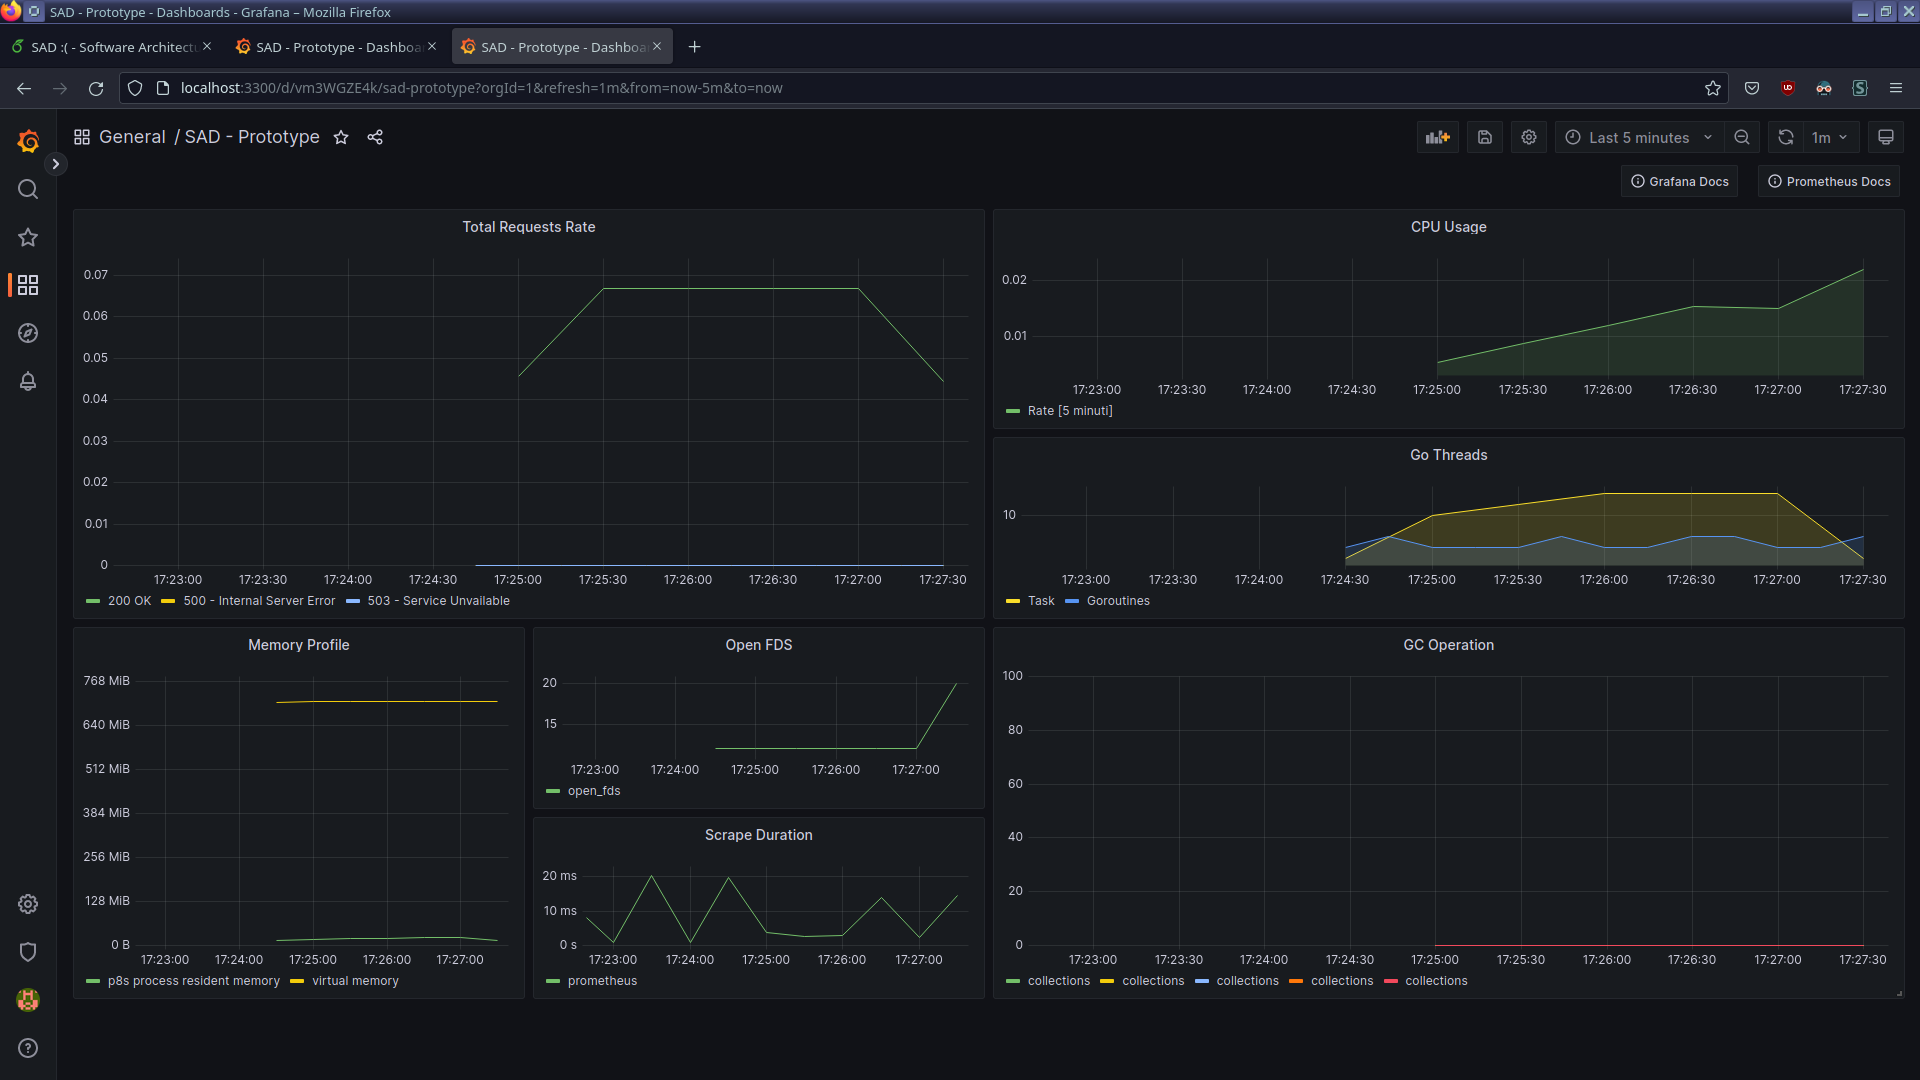
\includegraphics[width=\textwidth]{images/4Implementazione/grafana_dashboard.png}
    \caption{Esempio \textit{dashboard} Grafana}
    \label{fig:grafana_dashboard}
\end{figure}

\clearpage
\subsection{Paginazione}
Al fine di limitare la quantità di dati trasmessi nel caso di richieste che coinvolgono un grande numero di oggetti, come nel caso del recupero delle partite in un intervallo temporale, è stato implementato un meccanismo di paginazione di tipo \textit{skip and limit}. Questo tipo di procedura aggiunge due parametri alla richiesta da effettuare per recuperare i dati, come mostrato in \cref{fig:pagination1}:
\begin{itemize}
    \item \textbf{pageSize}: numero di oggetti recuperati per pagina; 
    \item \textbf{page}: numero di pagina;
\end{itemize}
In questo modo, supponendo di voler leggere alla pagina $p$ della tabella \textit{Game}, si otterranno $M$ record, in cui $m \in M$ sarà $(p-1) \cdot n\leq m \leq p \cdot n$. Inoltre, come mostrato in \cref{fig:pagination2}, la risposta viene arricchita con metadata utili a navigare le pagine in cui è stata divisa.


\begin{figure}[H]
    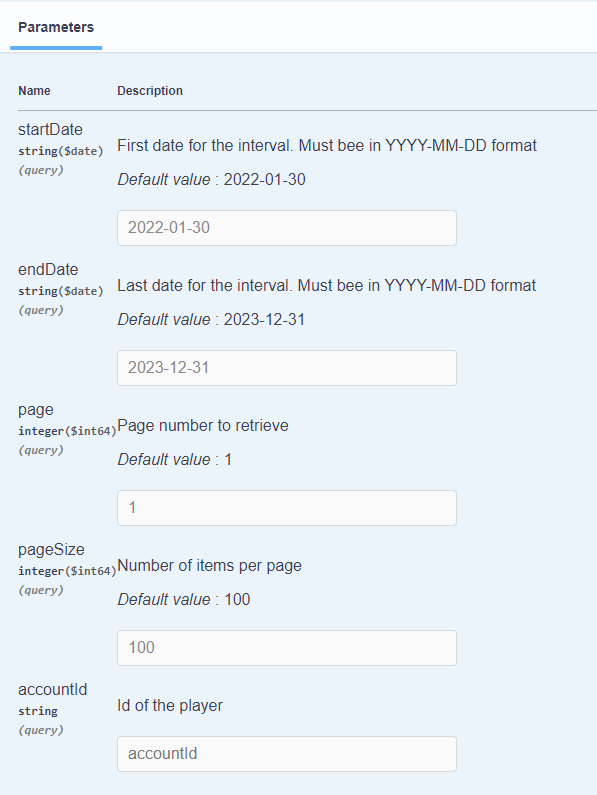
\includegraphics[width=.5\textwidth]{images/4Implementazione/pagination1.png}
    \centering
    \caption{Parametri richiesta con paginazione}
    \label{fig:pagination1}
\end{figure}

\begin{figure}[H]
    \centering
    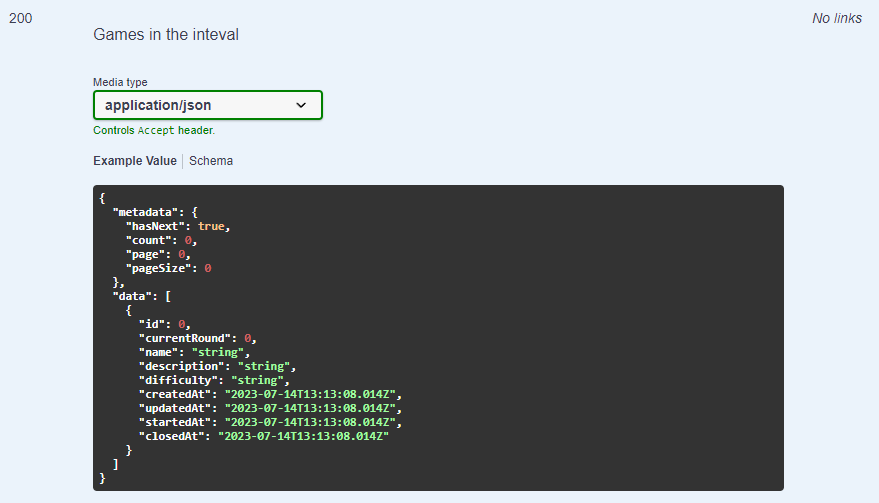
\includegraphics[width=.9\textwidth]{images/4Implementazione/pagination2.png}
    \caption{Risposta con paginazione}
    \label{fig:pagination2}
\end{figure}


\subsection{Rate limiting}
Per proteggere l'API da attacchi DDoS è stato predisposto un sistema di \textit{rate limiting} che implementa l'algoritmo \textit{\textbf{Token Bucket}}. Uno schema dell'algoritmo è mostrato in \cref{fig:rate_limiting}.

Questo componente è configurabile con 3 parametri:
\begin{itemize}
    \item Requests per seconds: numero di richieste al secondo prima di ottenere un errore;
    \item Bursts: numero di token presenti nel bucket, quando sono esauriti il client viene messo in attesa;
    \item Enabled: quando è impostato a \textit{False} il \textit{rate limiting} viene disattivato;
\end{itemize}

Il rate limiting viene applicato per client: per fare questo è stato aggiunta una funzione alla catena di \textit{middleware} dei controller che si occupa di recuperare l'ip dell'\textit{host} originale nel caso in cui l'applicazione sia preceduta da \textit{gateway} e/o \textit{reverse proxy}. Infatti, un'applicazione posizionata alle spalle di un \textit{reverse proxy}, ha come indirizzo sorgente delle richieste \textit{HTTP} quello del \textit{proxy} che per convenzione (per non perdere l'informazione) spostano all'interno di header standard quali \textit{X-Forwarded-For}, \textit{X-Real-IP} o \textit{True-Client-IP}.

\begin{figure}[H]
    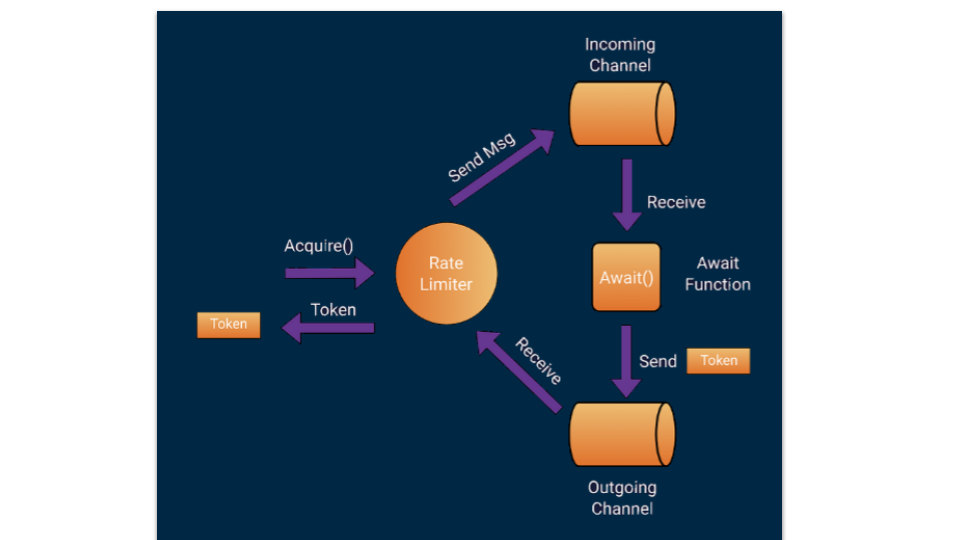
\includegraphics[width=\textwidth]{images/4Implementazione/rate_limiting.png}
    \caption{Algoritmo token bucket}
    \label{fig:rate_limiting}
\end{figure}

\clearpage
    
\section{Testing}
Il testing della soluzione avviene in maniera automatica ed è stato integrato nel ciclo di sviluppo e rilascio del software.
\subsection{Unit testing}
Il componente testato è il servizio REST descritto nei paragrafi precedenti. Per garantire una maggiore robustezza del sistema, l'oggetto principale del testing di unità è l'interfaccia input/output dell'applicazione. In particolare, con riferimento all'architettura mostrata in (aggiungere ref all'architettura), sono oggetto di questa attività i controller, ognuno dei quali viene testato con JSON sintatticamente validi verificando il risultato a un particolare codice dello standard HTTP. In questa fase, è stato utilizzato un approccio \textit{table testing} secondo cui per ogni componente è stata progettata una tabella di \textit{test case}, come mostrato in \cref{tab:unit_test}. 

\begin{table}[h]
    \centering
    \begin{tabular}{|l|l|c|}
        \hline
         TC & Descrizione & Risultato atteso (Codice HTTP) \\
        \hline
        \hline
         T01-GameNotExists & Ricerca di partita non esistente & 404 \\
        \hline
        T02-GameExists & Ricerca di partita esistente &  200 \\ 
        \hline
        T03-BadID & Ricerca partita con id invalido & 400\\
        \hline
        T11-BadJson  & Creazione partita con \textit{JSON} invalido & 400 \\
        \hline
        T12-GameCreated & Creazione partita con \textit{JSON} valido & 201 \\
        \hline  
    \end{tabular}
    \caption{Unit test effettuato per il \textit{Game Controller} }
    \label{tab:unit_test}
\end{table}

Attraverso, il sistema \textit{Make} è stato predisposto il \textit{target} \textbf{test} che oltre ad effettuare il testing di unità genera un file in cui vengono elaborate le metriche di copertura. In \cref{fig:unit_testing_example}, è mostrato un esempio di esecuzione del testing di unità.

\begin{figure}
    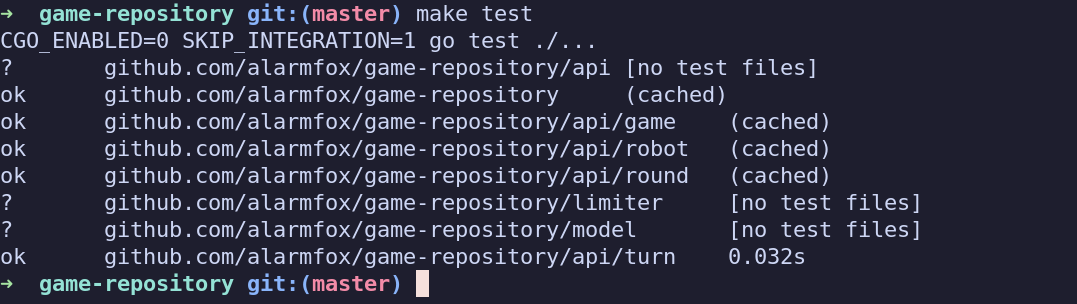
\includegraphics[width=\textwidth]{images/5Testing/unit_testing_output.png}
    \caption{Unit testing attraverso il comando \textit{make}}
    \label{fig:unit_testing_example}
\end{figure}


\subsection{Integration testing}
Il testing di integrazione mette insieme il componente REST Server con un'istanza di un \textit{database} reale. Con riferimento all'architettura della soluzione, sono state testate le funzioni del layer \textit{Service} che utilizza la base dati ed è utilizzata dai controller. In questa attività, l'obiettivo principale è quello di verificare la coerenza dei dati e la correttezza dello schema descritto in \cref{fig:er}.\\

Analogamente al testing di unità, è stato utilizzato l'approccio del \textit{table testing}. Ad esempio, per la procedura di salvataggio dei file appartenenti a un giocatore, è stata progettata la \cref{tab:int_test_save_file}. Dal punto di vista implementativo, la funzione riceve in ingresso:
\begin{itemize}
    \item \textbf{id}: identificativo del turno del giocatore rappresentato come intero a 64bit;
    \item \textbf{reader}: flusso di byte astratto dall'interfaccia \textit{io.Reader};
\end{itemize}

\begin{table}[h]
    \centering
    \begin{tabular}{|l|l|c|}
        \hline
         TC & Descrizione & Risultato atteso\\
        \hline
        \hline
         T51-NotAZip & Il corpo della richiesta non è uno zip & ErrNotAZip \\
        \hline
        T52-Success & Il file ZIP viene correttamente salvato &  OK\\ 
        \hline
         T53-EmptyFile & Il file ZIP è vuoto &  OK\\ 
        \hline
        T54-InvalidTurnID & L'ID del turno è negativo & ErrNotFound \\
        \hline
        T55-NullBody & Se l'ingresso ha valore NULL & ErrInvalidParam \\
        \hline
        T56-NotFound & Il turno non viene trovato all'interno del database & ErrNotFound \\
        \hline  
    \end{tabular}
    \caption{Unit test effettuato per la funzione \textit{SaveFile} del \textit{TurnService}}
    \label{tab:int_test_save_file}
\end{table}

Inoltre, per rendere predicibile il valore dei valori assegnati dal \textit{database} (ad esempio il valore delle sequenze per l'assegnazione degli ID quando viene effettuata una \textit{INSERT}) dopo ogni \textit{test case} viene eseguita l'operazione \textit{TRUNCATE} con lo scopo di effettuare il \textit{reset} di tutte le strutture del \textit{database} e rendere il \textit{testing} riproducibile.\\

In \cref{fig:int_testing_example}, è mostrato l'esecuzione del test di integrazione con il target \textit{test-integration}. In particolare, sono previsti alcuni parametri di configurazione:

\begin{itemize}
    \item \textit{CI=1}: attraverso il parametro \textit{DB\_URI} viene specificato un'istanza già esistente per il database. L'operazione comporta la perdita di dati;
    \item CI non specificato: viene creata un'istanza usa e getta del database con Docker;
\end{itemize}

\begin{figure}[H]
    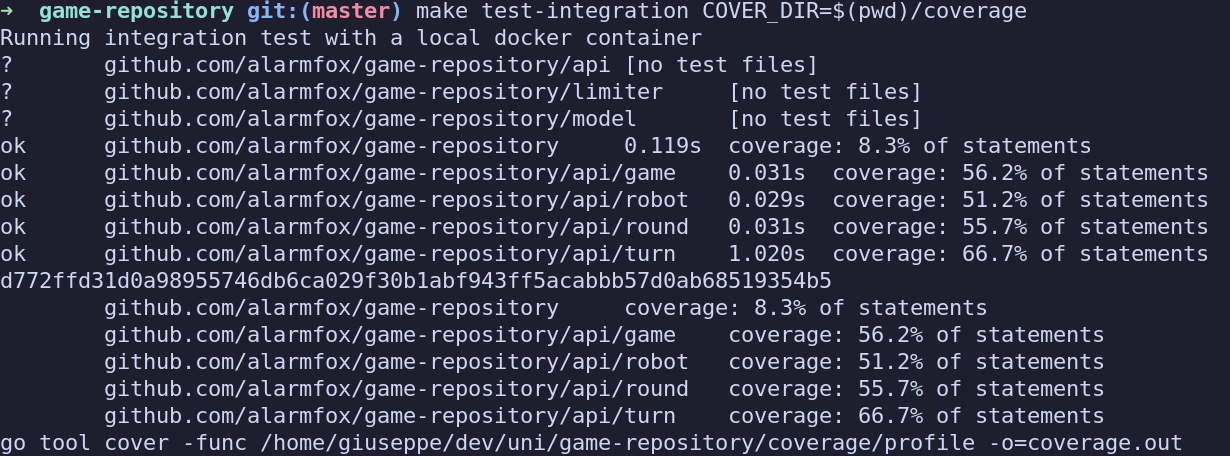
\includegraphics[width=\textwidth]{images/5Testing/int_testing_output.png}
    \caption{Esempio di esecuzione di \textit{integration testing} con il comando \textit{make}}
    \label{fig:int_testing_example}
\end{figure}

\section{Deployment}
In questa sezione, si fa riferimento all'installazione del solo componente \textit{Rest Server}; per gli altri componenti si rimanda alla guida ufficiale di installazione e configurazione. Tuttavia alla fine della sezione è comunque mostrata una versione completa del sistema installato e configurato con \textbf{docker-compose}.
Al fine di avere una soluzione completa funzionante, è necessario che tutti gli elementi dell'architettura si trovino all'interno della stessa rete. In generale, l'architettura per installare l'applicativo è illustrata nel \textit{deployment diagram} in \cref{fig:deployment_diagram}:

\begin{figure}[H]
    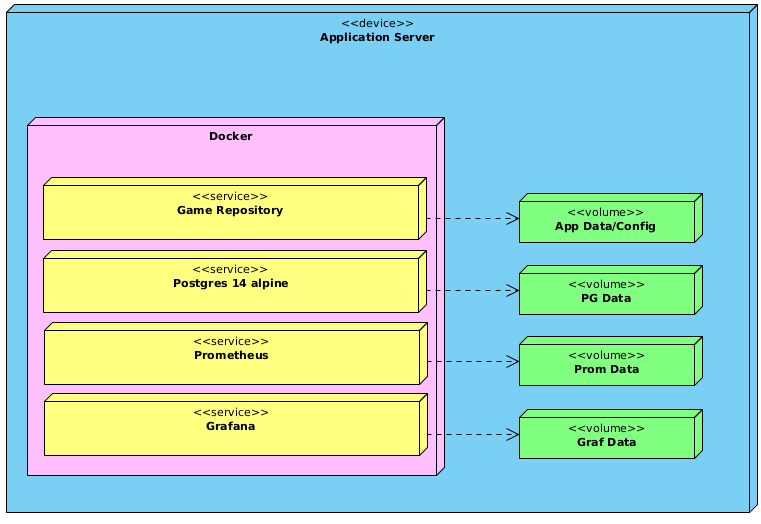
\includegraphics[width=\textwidth]{images/6Deployment/deployment_diagram.png}
    \caption{Deployment diagram della soluzione}
    \label{fig:deployment_diagram}
\end{figure}

\subsection{Configurazione}
L'applicazione si configura con un file JSON (obbligatorio anche se risulta vuoto) con la struttura riportata in \cref{lst:config} con i valori \textit{default} nel caso in cui non siano specificati. In particolare, l'applicazione cerca per un file chiamato \textit{config.json} nello stesso \textit{path} dell'eseguibile, ma è possibile specificare un percorso a scelta attraverso l'argomento CLI \textit{config=<PATH>}.


\begin{lstlisting}[
    language=json,
    firstnumber=1,
    caption={Struttura file di configurazione},
    label={lst:config}]
 {
    "postgresUrl": "",
    "listenAddress": "localhost:3000",
    "apiPrefix": "/",
    "dataPath": "data",
    "enableSwagger": false,
    "rateLimiting": {
        "enabled": false,
        "burst": 4,
        "maxRate": 2
    },
    "authentication": {
        "enabled": true,
        "headerKey": "Authorization",
        "authEndpoint": "http://auth-service/auth",
        "method": "POST"
    }
}
\end{lstlisting}

Gli oggetti \textit{rateLimiting} e \textit{authentication} abilitano i moduli opzionali come indicato nel paragrafo \cref{s:middleware}.


\subsection{Build System}
Il sistema di \textit{build} utilizzato è interamente basato su \textit{Make}. Per eseguire i comandi di compilazione è necessario avere un compilatore \textit{GO}. Di seguito sono illustrati le regole e gli obiettivi del \textit{Makefile} descritto per il progetto:
\begin{itemize}
    \item \textbf{build}: compila l'applicazione nella cartella specificata in \textit{OUT\_DIR} (che ha come default il valore "build");
    \item \textbf{run}: esegue l'applicazione compilata con l'obiettivo \textit{build}, con il file configurazione in \textit{CONFIG} (con valore di default "config.json");
    \item \textbf{dev}: avvia l'applicazione in modalità sviluppo (si riavvia ogni volta che viene modificato il codice sorgente). Prima di eseguire questa regola, eseguire il comando \textit{make dev-dependencies} che installerà \textit{air} (lo strumento che si occupera dell'operazione);
    \item \textbf{docker-build}: compila un'immagine Docker usando il tag \textit{game- repository: <GIT\_COMMIT>};
    \item \textbf{docker-run}: esegue l'immagine in un container usando il parametro \textit{CONFIG}, analogamente allo step \textit{run};
    \item \textbf{docker-push-ssh}: invia l'immagine ad un server utilizzando il protocollo SSH. I parametri per la connessione attraverso SSH devono essere passati attraverso la variabile \textit{SSH} (vuota di default);
    \item \textbf{docker-push}: invia l'immagine ad un \textit{docker registry}. Il nome del \textit{registry} viene specificato nella variabile \textit{REGISTRY}. In particolare, viene fatto l'invio dell'immagine sia con il tag pari al git commit sia che come \textit{latest};
    \item \textbf{test}: viene effettuato il test unità dell'applicazione;
    \item \textbf{test-integration} (linux-only): viene effettuato il test di integrazione dell'applicazione. In particolare, se il flag \textit{CI} viene specificato, è possibile usare la variabile \textit{DB\_URI} per specificare l'indirizzo di un \textit{database} di test, altrimenti sarà un database usa e getta attraverso un \textit{Docker container}. Inoltre, attraverso la variabile \textit{COVER\_DIR} la cartella in cui sarà salvato il file per le metriche di copertura;
    \item \textbf{clean}: rimuove gli artefatti prodotti;
    \item \textbf{help}: utilizza i commenti nel \textit{Makefile} per creare una piccola guida all'utilizzo con esempi di utilizzo;
\end{itemize}

\subsection{Modalità di deploy}
\subsubsection{Standalone}
La modalità di installazione più semplice è quella \textit{standalone}. L'applicazione è compilata in un singolo file eseguibile che può essere compilato direttamente dal codice sorgente (usando il comando \textit{make build}) oppure può essere scaricato dalla sezione \textit{release} del progetto (si rimanda al paragrafo \cref{s:cicd} per una spiegazione esaustiva). 

\subsubsection{Docker}
L'applicazione può essere installata compilando un'immagine Docker per essere eseguita in un \textit{container}. La procedura di compilazione è ottimizzata utilizzando il \textit{multi-stage building} dell'immagine con l'adozione del sistema operativo \textit{alpine} ottenendo un'immagine di circa 25MB. Analogamente al caso \textit{standalone}, l'immagine può essere compilata sia dal codice sorgente (con il comando \textit{make docker-build}), oppure è possibile scaricarne una già pronta dal \textit{repository capas/game-repository}

\paragraph{Esempio di applicazione completa con docker-compose}
Docker compose è un'applicazione che serve ad installare \textit{stack} applicativi  (configurati in file in formato \textit{yaml}) provvedendo a fornire per ogni applicazione servizi di utilità, come mostrato nell'elenco di seguito (non esaustivo):
\begin{itemize}
    \item Servizi di rete: docker-compose crea una rete dedicata per ogni stack e offre (in base al nome specificato per l'applicazione) un servizio DNS;
    \item Dipendenze tra i servizi: i servizi possono dipendere tra loro e questo consente di decidere l'ordine di avvio;
    \item Sistema di healthcheck: specificato un comando, un servizio può essere marcato come "in salute" oppure "mancante";
    \item Politiche di riavvio: un'applicazione può essere riavviata ogni volta che c'è un crash per un numero definito di volte ecc;
\end{itemize}

In è mostrato un \textit{docker-compose.yml} funzionanete per installare l'applicazione come mostrato in \cref{fig:deployment_diagram}.

\begin{lstlisting}[
    style=yaml,
    firstnumber=1,
    caption={Docker compose applicazione funzionante},
    label={lst:docker_compose}]
version: '3'

volumes:
  pgdata:
  appdata:
  grafdata:
  promdata:

services:
  app:
    image: capas/game-repository:latest
    ports:
      - 3000:3000/tcp
    volumes:
      - appdata:/app/data
      - ./config.docker.json:/app/config.json
    depends_on:
      - db
  db:
    image: postgres:14-alpine3.17
    environment:
      POSTGRES_PASSWORD: postgres
    volumes:
      - pgdata:/var/lib/postgresql/data
    healthcheck:
      test: ["CMD-SHELL", "pg_isready", "-d", "postgres"]
      interval: 30s
      timeout: 60s
      retries: 5
      start_period: 80s

  prometheus:
    image: prom/prometheus
    volumes:
      - ./prometheus.yml:/etc/prometheus/prometheus.yml
      # reference https://github.com/prometheus/prometheus/blob/main/Dockerfile
      - promdata:/prometheus
    ports:
      - 3330:9090

  grafana:
    image: grafana/grafana
    ports:
      - 3300:3000/tcp
    volumes:
      - grafdata:/var/lib/grafana

  
\end{lstlisting}

\subsection{CI/CD}\label{s:cicd}
Con l'utilizzo di \textit{Github Actions}, è stato automatizzato il processo di \textit{testing} per essere eseguito prima di ogni azione sul \textit{branch} \textbf{master} (\textit{push}, \textit{pull request}) per garantire uno standard minimo per la qualità del software. In particolare, ad ogni operazione viene aggiornato il file \textit{README.md} con informazioni riguardanti la copertura delle righe di codice, lo stato dell'ultima esecuzione e il risultato dell'analisi statica del codice (ottenuta grazie all'utilizzo del servizio \textit{Go Report Card}\cite{goreport}) sotto forma di \textit{badge}, come mostrato in \cref{fig:ci_badge}.

\begin{figure}[H]
    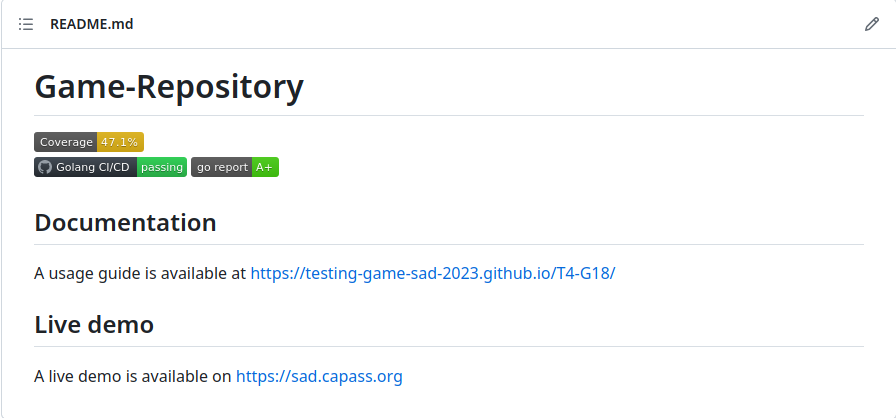
\includegraphics[width=\textwidth]{images/5Testing/ci_badge.png}
    \caption{Badge ottenuti dopo l'esecuzione della \textit{pipeline} CI/CD}
    \label{fig:ci_badge}
\end{figure}

Inoltre, è stato implementata la \textit{Continous Delivery} attraverso \textit{Github Actions} che viene attivata alla creazione di una \textit{release}. All'attivazione dello script vengono eseguite le seguenti operazioni:
\begin{itemize}
    \item Test: il \textit{branch} scelto per la \textit{release} viene testato (sia con test di unità e integrazione). Se questo passo fallisce, il rilascio non viene effettuato;
    \item Build con Docker: viene creata un'immagine Docker che viene salvata sul \textit{repository} pubblico \textit{capas/game-repository};
    \item Deploy della versione live: con SSH, viene aggiornata l'applicazione sul server;
    \item Pubblicazione di \textit{artifact}: con riferimento alla matrice architettura/sistema operativo in \cref{tab:comp_matrix}, per ciascuna cella supportata viene creato un archivio contenente: l'eseguibile, file di licenza, README.md, specifica OpenAPI e una collection Postman per gli facilitare l'integrazione con gli altri componenti;
\end{itemize}

\begin{table}[h]
    \centering
    \begin{tabular}{|l|l|l|l|l|}
        \hline
         Arch/OS & Linux & Windows & Darwin \\
        \hline
        \hline
         i386 & x & x &  \\
         amd64 & x & x & x \\
         arm64 & x & & x  \\
        \hline
    \end{tabular}
    \caption{Matrice di compatibilità supportata}
    \label{tab:comp_matrix}
\end{table}

\begin{figure}[H]
    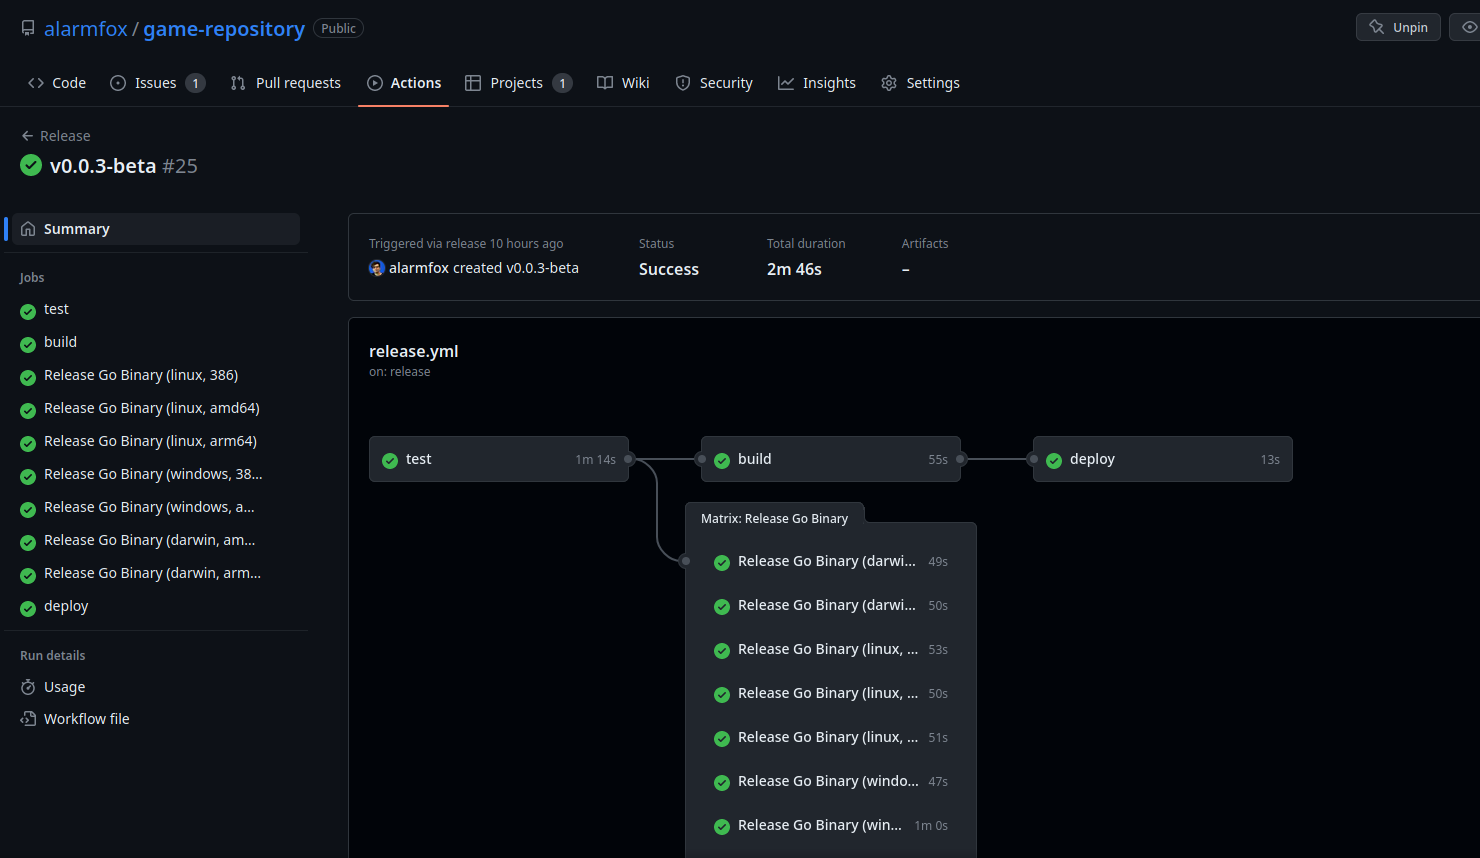
\includegraphics[width=\textwidth]{images/6Deployment/cd.png}
    \caption{Esecuzione dello script CD per la release 0.0.3-beta}
    \label{fig:cd}
\end{figure}

\paragraph{Documentazione online}
Con lo scopo di rendere la \textit{repository} \textit{self-contained}, l'applicazione offre una documentazione contenente una guida pratica all'installazione che viene compilata da una \textit{Github Action}. In particolare, questa documentazione è generata con \textit{mkdocs}\cite{mkdocs} che consente di passare da semplici file di testo in \textit{Markdown} a \textit{HTML}. Un esempio di documentazione è mostrato in \cref{fig:docs}.

\begin{figure}[H]
    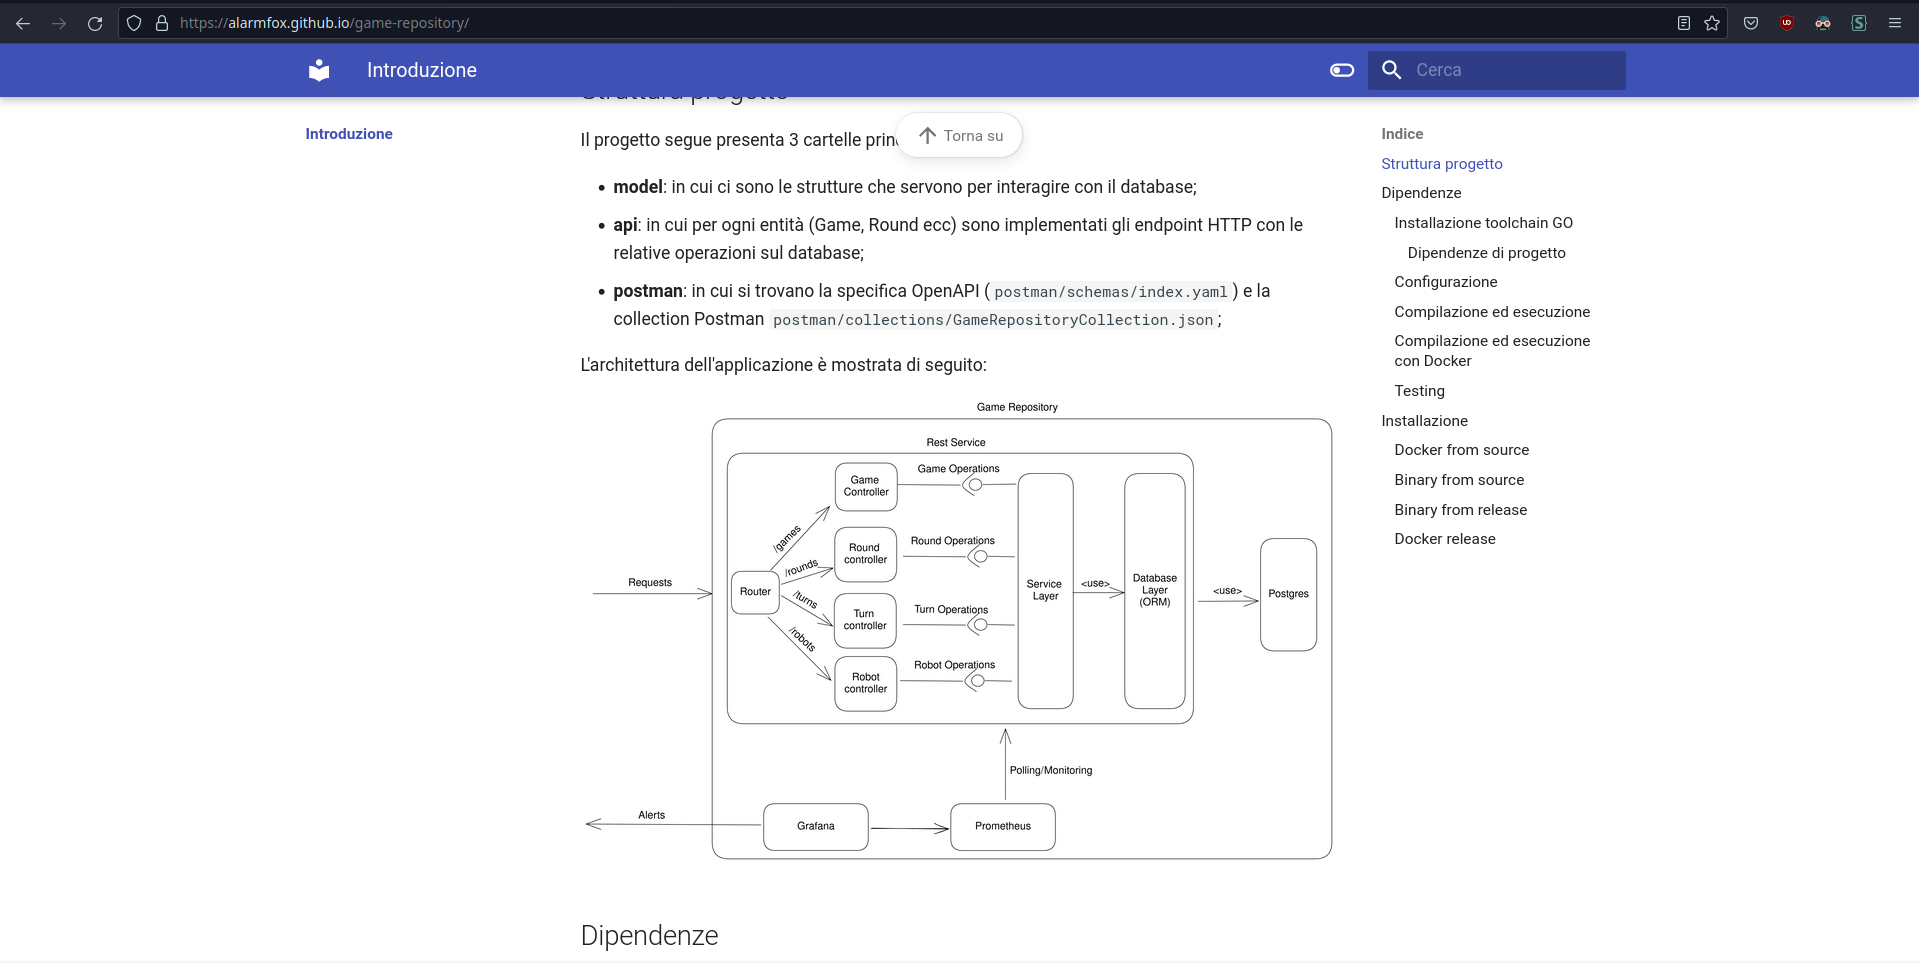
\includegraphics[width=\textwidth]{images/6Deployment/docs.png}
    \caption{Screenshot della documentazione online}
    \label{fig:docs}
\end{figure}

La documentazione è consultabile al link indicato in \cref{s:links}.

\subsection{Integrazione con altri componenti}
Essendo uno dei task con minori dipendenze e al servizio degli altri si è cercato da subito di fornire una chiara lista dei servizi messi a disposizione, interfacciandosi con i membri degli altri team. 
Di seguito la lista dei gruppi con il relativo task a cui sono state fornite direttamente le API e la documentazione di supporto:
\begin{itemize}
    \item Gruppo 14 , Task 5
    \item Gruppo 5, Task 5
    \item Gruppo 8, Task 6   
\end{itemize}

Coordinandosi con il gruppo G4 (task 4), nonostante le differenti tecnologie adoperate, si è scelto  di esporre un'interfaccia per lo più identica, in modo che gli altri team di sviluppo potessero scegliere liberamente tra le due versioni, ma che non ci fossero discrepanze eccessive. 


\subsubsection{Infrastruttura di laboratorio}
Il gruppo ha fornito supporto nella creazione dell'infrastruttura del laboratorio permettendo di creare diverse istanze dell'applicazione completa in cui i singoli componenti sviluppati da team indipendenti possono comunicare fra loro. In particolare, l'architettura da utilizzare è a microservizi disponendo di una macchina Windows 11 con 5 utenze dedicate all'applicazione denominate \textbf{Testing Game X} (con $X$ da 1 a 5).\\

Lo scopo dell'attività è stato quello di creare, per ciascuna utenza una rete e un volume virtuale con Docker. Ogni rete è stata denominata con \textbf{testing-game-nw-x} (con $x$ da 1 a 5); mentre ogni volume \textbf{testing-game-data-x} (con $x$ da 1 a 5). In questo modo, ogni utente può effettuare il \textit{deploy} del proprio stack applicativo attraverso \textit{docker-compose} e collegare i container che devono essere in comunicazione nella rete dedicata. Per facilitare l'operazione, è stato creato un template per \textit{docker-compose} in cui sono già dichiarati i volumi e le reti da collegare ai servizi. Inoltre, l'utilizzo di una rete comune può essere utilizzata per condividere istanze di componenti comuni. Ad esempio, se più gruppi utilizzano \textit{MongoDB} è possibile crearne un'istanza nella rete \textit{testing-game-nw-x} e condividerla tra i diversi stack.

\begin{figure}[H]
    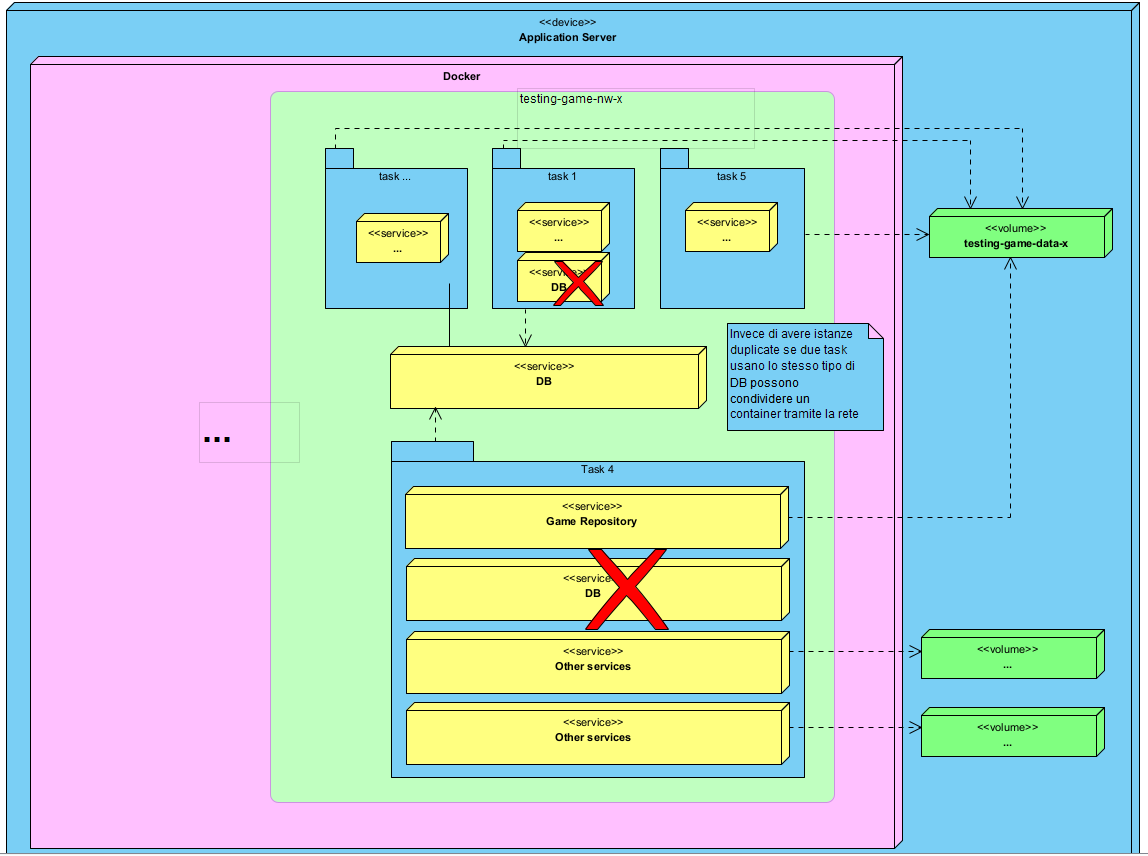
\includegraphics[width=\textwidth]{images/6Deployment/networks.png}
    \caption{Deploy con network e DB condiviso}
    \label{fig:network-deploy}
\end{figure}

Il template è riportato di seguito per semplicità.

\begin{lstlisting}[
    style=yaml,
    firstnumber=1,
    caption={Docker compose applicazione funzionante},
    label={lst:template}]
version: '3'

volumes:
  # sostituire alla "x" il numero dell'utente scelto
  testing-game-data-x:
    external: true
  # aggiungere eventuali altri volumi
  # ....

networks:
  # sostituire alla "x" il numero dell'utente scelto
  testing-game-nw-x:
    external: true
  # aggiungere eventuali altre reti
  # ....

# A titolo di esempio e' mostrata una classica applicazione con servizio + database
services:
  app:
    image: <image>
    ports:
      - <host-port>:<container-port>
    volumes:
      # dati da condividere con gli altri container
      - testing-game-data-x:/path/ai/dati/nel/container
      # altri volumi ...
    networks:
      # sostituire x con il nome dell'utente
      - testing-game-nw-x
      # ATTENZIONE: affinche' l'applicazione comunichi con il database local
      # e' necessario inserirla nella rete "default" creata da
      # docker-compose
      - default
    # completare la configurazione con eventuali parametri
    # ...
    depends_on:
      - db

  db:
    image: postgres:14-alpine3.17
    environment:
      POSTGRES_PASSWORD: postgres
      # altri parametri di configurazione...
    volumes:
      # eventuale volume per la persistenza dei dati del database
      - <volume>:/var/lib/postgresql/data
    # questa sezione serve ad assicurarsi che il database sia inizializzato correttamente
    # prima di avviare l'applicazione
    healthcheck:
      test: ["CMD-SHELL", "pg_isready", "-d", "postgres"]
      interval: 30s
      timeout: 60s
      retries: 5
      start_period: 80s
\end{lstlisting}

\clearpage
\printbibliography

\end{document}
